% Generated fragments require trusted human review before compilation.
% This binder never requests shell escape or runs external tools.
\documentclass[11pt]{article}
% Trusted shared apparatus. Requires LuaLaTeX; never use shell escape.
\usepackage{fontspec}
\defaultfontfeatures{Ligatures=TeX}
\IfFontExistsTF{Noto Serif}{\setmainfont{Noto Serif}}{%
  \IfFontExistsTF{DejaVu Serif}{\setmainfont{DejaVu Serif}}{%
    \IfFontExistsTF{Times New Roman}{\setmainfont{Times New Roman}}{%
      \PackageError{gelfand-binder}{No configured Cyrillic serif font installed}{Install Noto Serif or DejaVu Serif, or select an installed Cyrillic font.}%
    }%
  }%
}
\IfFontExistsTF{Noto Sans}{\setsansfont{Noto Sans}}{%
  \IfFontExistsTF{DejaVu Sans}{\setsansfont{DejaVu Sans}}{\setsansfont{Arial}}%
}
\IfFontExistsTF{Noto Sans Mono}{\setmonofont{Noto Sans Mono}}{%
  \IfFontExistsTF{DejaVu Sans Mono}{\setmonofont{DejaVu Sans Mono}}{\setmonofont{Courier New}}%
}
\usepackage[a4paper,margin=22mm]{geometry}
\usepackage{amsmath,amssymb,amsthm,mathtools}
\usepackage{xcolor}
\usepackage{tikz}
\usepackage{tikz-cd}
\usetikzlibrary{arrows.meta,positioning,calc}
\usepackage{hyperref}
\hypersetup{unicode=true,colorlinks=true,linkcolor=blue,pdftitle={Gelfand transcription binder}}
\newtheorem{theorem}{Theorem}
\newtheorem{lemma}{Lemma}
\newtheorem{proposition}{Proposition}
\newtheorem{corollary}{Corollary}
\theoremstyle{definition}
\newtheorem{definition}{Definition}
\newtheorem{example}{Example}
\theoremstyle{remark}
\newtheorem{remark}{Remark}
\setlength{\parindent}{0pt}
\setlength{\parskip}{0.55em}
\setlength{\emergencystretch}{3em}
\newcommand{\SourcePage}[2]{%
  \clearpage\phantomsection\label{#1:source-page}%
  \addcontentsline{toc}{subsection}{#1}%
  {\small\sffamily\color{blue!60!black}Source scan frame: #1; visible page/leaf label: #2}\par\medskip%
}
\newcommand{\Unclear}[3]{%
  \begingroup\color{orange!70!black}%
  [Unresolved reading #1/#2: #3]\endgroup%
}
\newcommand{\Incomplete}[3]{%
  \par\begingroup\color{red!65!black}\textbf{Incomplete #1/#2:} #3\endgroup\par%
}
\newcommand{\SourceFigure}[3]{%
  \par\begingroup\color{blue!60!black}\textbf{\hyperref[#1:source-page]{Source figure #1/#2}:} #3%
  \par\textit{Consult the authoritative scan at this locator.}\endgroup\par%
}



% Reader layout only. Original diplomatic text is retained verbatim.
\setlength{\parskip}{0.35em}
\setlength{\emergencystretch}{4em}
\renewcommand{\SourcePage}[2]{%
  \par\addvspace{1em}\phantomsection\label{#1:source-page}%
  \addcontentsline{toc}{subsection}{#1}%
  {\footnotesize\sffamily\color{blue!55!black}#1%
    \def\givenlabel{#2}\def\nolabel{unlabelled}%
    \ifx\givenlabel\nolabel\else\quad[номер в источнике: #2]\fi
  }\par\nobreak\smallskip%
}
\renewcommand{\Unclear}[3]{%
  \begingroup\color{orange!65!black}%
  \ifmmode\text{[неясно: #3]}\else[неясно: #3]\fi\endgroup%
}
\renewcommand{\Incomplete}[3]{%
  \par\begingroup\color{red!60!black}\textbf{Неразобранный фрагмент:} #3%
  \endgroup\par%
}
\renewcommand{\SourceFigure}[3]{%
  \par\begingroup\color{blue!55!black}\textbf{Рисунок:} #3%
  \par{\small\textit{Исходный рисунок: \hyperref[#1:source-page]{#1}, #2.}}%
  \endgroup\par%
}
\hypersetup{pdftitle={Семинар И. М. Гельфанда. Дипломатическая транскрипция},pdfauthor={},pdfsubject={Русское рабочее издание с отмеченными сомнительными чтениями}}

\usepackage[normalem]{ulem}
\usepackage{newunicodechar}
\usepackage{adjustbox}
\newfontfamily\SourceSymbolFont{Segoe UI Symbol}
\newfontfamily\SourceCJKFont{MS Gothic}
\let\DiplomaticMathUnderline\underline
\renewcommand{\underline}[1]{\ifmmode\DiplomaticMathUnderline{#1}\else\uline{#1}\fi}
\newunicodechar{→}{\ifmmode\text{{\SourceSymbolFont\char"2192}}\else{\SourceSymbolFont\char"2192}\fi}
\newunicodechar{⇒}{\ifmmode\text{{\SourceSymbolFont\char"21D2}}\else{\SourceSymbolFont\char"21D2}\fi}
\newunicodechar{∀}{\ifmmode\text{{\SourceSymbolFont\char"2200}}\else{\SourceSymbolFont\char"2200}\fi}
\newunicodechar{∂}{\ifmmode\text{{\SourceSymbolFont\char"2202}}\else{\SourceSymbolFont\char"2202}\fi}
\newunicodechar{∈}{\ifmmode\text{{\SourceSymbolFont\char"2208}}\else{\SourceSymbolFont\char"2208}\fi}
\newunicodechar{∌}{\ifmmode\text{{\SourceSymbolFont\char"220C}}\else{\SourceSymbolFont\char"220C}\fi}
\newunicodechar{√}{\ifmmode\text{{\SourceSymbolFont\char"221A}}\else{\SourceSymbolFont\char"221A}\fi}
\newunicodechar{∞}{\ifmmode\text{{\SourceSymbolFont\char"221E}}\else{\SourceSymbolFont\char"221E}\fi}
\newunicodechar{∧}{\ifmmode\text{{\SourceSymbolFont\char"2227}}\else{\SourceSymbolFont\char"2227}\fi}
\newunicodechar{∩}{\ifmmode\text{{\SourceSymbolFont\char"2229}}\else{\SourceSymbolFont\char"2229}\fi}
\newunicodechar{∪}{\ifmmode\text{{\SourceSymbolFont\char"222A}}\else{\SourceSymbolFont\char"222A}\fi}
\newunicodechar{∫}{\ifmmode\text{{\SourceSymbolFont\char"222B}}\else{\SourceSymbolFont\char"222B}\fi}
\newunicodechar{∴}{\ifmmode\text{{\SourceSymbolFont\char"2234}}\else{\SourceSymbolFont\char"2234}\fi}
\newunicodechar{∼}{\ifmmode\text{{\SourceSymbolFont\char"223C}}\else{\SourceSymbolFont\char"223C}\fi}
\newunicodechar{≈}{\ifmmode\text{{\SourceSymbolFont\char"2248}}\else{\SourceSymbolFont\char"2248}\fi}
\newunicodechar{≠}{\ifmmode\text{{\SourceSymbolFont\char"2260}}\else{\SourceSymbolFont\char"2260}\fi}
\newunicodechar{≤}{\ifmmode\text{{\SourceSymbolFont\char"2264}}\else{\SourceSymbolFont\char"2264}\fi}
\newunicodechar{≥}{\ifmmode\text{{\SourceSymbolFont\char"2265}}\else{\SourceSymbolFont\char"2265}\fi}
\newunicodechar{⊕}{\ifmmode\text{{\SourceSymbolFont\char"2295}}\else{\SourceSymbolFont\char"2295}\fi}
\newunicodechar{⊗}{\ifmmode\text{{\SourceSymbolFont\char"2297}}\else{\SourceSymbolFont\char"2297}\fi}
\newunicodechar{①}{\ifmmode\text{{\SourceSymbolFont\char"2460}}\else{\SourceSymbolFont\char"2460}\fi}
\newunicodechar{②}{\ifmmode\text{{\SourceSymbolFont\char"2461}}\else{\SourceSymbolFont\char"2461}\fi}
\newunicodechar{③}{\ifmmode\text{{\SourceSymbolFont\char"2462}}\else{\SourceSymbolFont\char"2462}\fi}
\newunicodechar{④}{\ifmmode\text{{\SourceSymbolFont\char"2463}}\else{\SourceSymbolFont\char"2463}\fi}
\newunicodechar{Ⓗ}{\ifmmode\text{{\SourceSymbolFont\char"24BD}}\else{\SourceSymbolFont\char"24BD}\fi}
\newunicodechar{〃}{\ifmmode\text{{\SourceCJKFont\char"3003}}\else{\SourceCJKFont\char"3003}\fi}


% Reader revision 3. Annotation wording and candidates remain unchanged.
\usetikzlibrary{shapes.geometric,decorations.pathreplacing,decorations.markings,patterns,fit}
\newsavebox{\ReaderAnnotationBox}
\newcommand{\ReaderAnnotation}[1]{%
  \sbox{\ReaderAnnotationBox}{[неясно: #1]}%
  \ifdim\wd\ReaderAnnotationBox>.70\linewidth
    \parbox[t]{.70\linewidth}{\raggedright[неясно: #1]}%
  \else\usebox{\ReaderAnnotationBox}\fi%
}
\ExplSyntaxOn
\cs_new_protected:Npn \reader_unclear_candidate:n #1
 {
  \tl_set:Nx \l_tmpa_tl { \tl_to_str:n {#1} }
  % Text explicitly guarded inside a mathematical candidate remains math-safe.
  \regex_replace_all:nnN { \\(?:text|textrm|textnormal|textbf|operatorname)\s*\{[^{}]*\} } { } \l_tmpa_tl
  \regex_match:nVTF { [\x{0400}-\x{052F}] | \$ } \l_tmpa_tl
   { \ifmmode \text{\ReaderAnnotation{#1}} \else \ReaderAnnotation{#1} \fi }
   {
    \ifmmode
      [\text{неясно:~}#1]
    \else
      \regex_match:nVTF { [_^] | \\ } \l_tmpa_tl
       { \ensuremath{[\text{неясно:~}#1]} }
       { \ReaderAnnotation{#1} }
    \fi
   }
 }
\RenewDocumentCommand \Unclear { m m m }
 { \begingroup\color{orange!65!black}\reader_unclear_candidate:n{#3}\endgroup }
\ExplSyntaxOff
\newsavebox{\ReaderIncompleteBox}
\newcommand{\ReaderIncompleteNote}[1]{%
 \sbox{\ReaderIncompleteBox}{\textbf{Неразобранный фрагмент:} #1}%
 \ifdim\wd\ReaderIncompleteBox>.70\linewidth
  \parbox[t]{.70\linewidth}{\raggedright\textbf{Неразобранный фрагмент:} #1}%
 \else\usebox{\ReaderIncompleteBox}\fi%
}
\renewcommand{\Incomplete}[3]{%
 \ifmmode\text{\color{red!60!black}\ReaderIncompleteNote{#3}}%
 \else\par\begingroup\color{red!60!black}\textbf{Неразобранный фрагмент:} #3\endgroup\par\fi%
}
% Ragged right avoids stretching long untranslated abbreviations into margins.
\AtBeginDocument{\raggedright}
\newunicodechar{А}{\ifmmode\text{\char"410\relax}\else\char"410\relax\fi}
\newunicodechar{Б}{\ifmmode\text{\char"411\relax}\else\char"411\relax\fi}
\newunicodechar{В}{\ifmmode\text{\char"412\relax}\else\char"412\relax\fi}
\newunicodechar{Г}{\ifmmode\text{\char"413\relax}\else\char"413\relax\fi}
\newunicodechar{Д}{\ifmmode\text{\char"414\relax}\else\char"414\relax\fi}
\newunicodechar{Е}{\ifmmode\text{\char"415\relax}\else\char"415\relax\fi}
\newunicodechar{Ж}{\ifmmode\text{\char"416\relax}\else\char"416\relax\fi}
\newunicodechar{З}{\ifmmode\text{\char"417\relax}\else\char"417\relax\fi}
\newunicodechar{И}{\ifmmode\text{\char"418\relax}\else\char"418\relax\fi}
\newunicodechar{Й}{\ifmmode\text{\char"419\relax}\else\char"419\relax\fi}
\newunicodechar{К}{\ifmmode\text{\char"41A\relax}\else\char"41A\relax\fi}
\newunicodechar{Л}{\ifmmode\text{\char"41B\relax}\else\char"41B\relax\fi}
\newunicodechar{М}{\ifmmode\text{\char"41C\relax}\else\char"41C\relax\fi}
\newunicodechar{Н}{\ifmmode\text{\char"41D\relax}\else\char"41D\relax\fi}
\newunicodechar{О}{\ifmmode\text{\char"41E\relax}\else\char"41E\relax\fi}
\newunicodechar{П}{\ifmmode\text{\char"41F\relax}\else\char"41F\relax\fi}
\newunicodechar{Р}{\ifmmode\text{\char"420\relax}\else\char"420\relax\fi}
\newunicodechar{С}{\ifmmode\text{\char"421\relax}\else\char"421\relax\fi}
\newunicodechar{Т}{\ifmmode\text{\char"422\relax}\else\char"422\relax\fi}
\newunicodechar{У}{\ifmmode\text{\char"423\relax}\else\char"423\relax\fi}
\newunicodechar{Ф}{\ifmmode\text{\char"424\relax}\else\char"424\relax\fi}
\newunicodechar{Х}{\ifmmode\text{\char"425\relax}\else\char"425\relax\fi}
\newunicodechar{Ц}{\ifmmode\text{\char"426\relax}\else\char"426\relax\fi}
\newunicodechar{Ч}{\ifmmode\text{\char"427\relax}\else\char"427\relax\fi}
\newunicodechar{Ш}{\ifmmode\text{\char"428\relax}\else\char"428\relax\fi}
\newunicodechar{Щ}{\ifmmode\text{\char"429\relax}\else\char"429\relax\fi}
\newunicodechar{Ъ}{\ifmmode\text{\char"42A\relax}\else\char"42A\relax\fi}
\newunicodechar{Ы}{\ifmmode\text{\char"42B\relax}\else\char"42B\relax\fi}
\newunicodechar{Ь}{\ifmmode\text{\char"42C\relax}\else\char"42C\relax\fi}
\newunicodechar{Э}{\ifmmode\text{\char"42D\relax}\else\char"42D\relax\fi}
\newunicodechar{Ю}{\ifmmode\text{\char"42E\relax}\else\char"42E\relax\fi}
\newunicodechar{Я}{\ifmmode\text{\char"42F\relax}\else\char"42F\relax\fi}
\newunicodechar{а}{\ifmmode\text{\char"430\relax}\else\char"430\relax\fi}
\newunicodechar{б}{\ifmmode\text{\char"431\relax}\else\char"431\relax\fi}
\newunicodechar{в}{\ifmmode\text{\char"432\relax}\else\char"432\relax\fi}
\newunicodechar{г}{\ifmmode\text{\char"433\relax}\else\char"433\relax\fi}
\newunicodechar{д}{\ifmmode\text{\char"434\relax}\else\char"434\relax\fi}
\newunicodechar{е}{\ifmmode\text{\char"435\relax}\else\char"435\relax\fi}
\newunicodechar{ж}{\ifmmode\text{\char"436\relax}\else\char"436\relax\fi}
\newunicodechar{з}{\ifmmode\text{\char"437\relax}\else\char"437\relax\fi}
\newunicodechar{и}{\ifmmode\text{\char"438\relax}\else\char"438\relax\fi}
\newunicodechar{й}{\ifmmode\text{\char"439\relax}\else\char"439\relax\fi}
\newunicodechar{к}{\ifmmode\text{\char"43A\relax}\else\char"43A\relax\fi}
\newunicodechar{л}{\ifmmode\text{\char"43B\relax}\else\char"43B\relax\fi}
\newunicodechar{м}{\ifmmode\text{\char"43C\relax}\else\char"43C\relax\fi}
\newunicodechar{н}{\ifmmode\text{\char"43D\relax}\else\char"43D\relax\fi}
\newunicodechar{о}{\ifmmode\text{\char"43E\relax}\else\char"43E\relax\fi}
\newunicodechar{п}{\ifmmode\text{\char"43F\relax}\else\char"43F\relax\fi}
\newunicodechar{р}{\ifmmode\text{\char"440\relax}\else\char"440\relax\fi}
\newunicodechar{с}{\ifmmode\text{\char"441\relax}\else\char"441\relax\fi}
\newunicodechar{т}{\ifmmode\text{\char"442\relax}\else\char"442\relax\fi}
\newunicodechar{у}{\ifmmode\text{\char"443\relax}\else\char"443\relax\fi}
\newunicodechar{ф}{\ifmmode\text{\char"444\relax}\else\char"444\relax\fi}
\newunicodechar{х}{\ifmmode\text{\char"445\relax}\else\char"445\relax\fi}
\newunicodechar{ц}{\ifmmode\text{\char"446\relax}\else\char"446\relax\fi}
\newunicodechar{ч}{\ifmmode\text{\char"447\relax}\else\char"447\relax\fi}
\newunicodechar{ш}{\ifmmode\text{\char"448\relax}\else\char"448\relax\fi}
\newunicodechar{щ}{\ifmmode\text{\char"449\relax}\else\char"449\relax\fi}
\newunicodechar{ъ}{\ifmmode\text{\char"44A\relax}\else\char"44A\relax\fi}
\newunicodechar{ы}{\ifmmode\text{\char"44B\relax}\else\char"44B\relax\fi}
\newunicodechar{ь}{\ifmmode\text{\char"44C\relax}\else\char"44C\relax\fi}
\newunicodechar{э}{\ifmmode\text{\char"44D\relax}\else\char"44D\relax\fi}
\newunicodechar{ю}{\ifmmode\text{\char"44E\relax}\else\char"44E\relax\fi}
\newunicodechar{я}{\ifmmode\text{\char"44F\relax}\else\char"44F\relax\fi}
\newunicodechar{Ё}{\ifmmode\text{\char"401\relax}\else\char"401\relax\fi}
\newunicodechar{ё}{\ifmmode\text{\char"451\relax}\else\char"451\relax\fi}


% Reader-only pairing support; accepted raw bodies remain unchanged.
\RequirePackage{graphicx}
\RequirePackage{adjustbox}
\newcommand{\ReaderOriginalPanel}[2]{%
  \begin{minipage}[t]{.48\linewidth}\vspace{0pt}\centering
    \includegraphics[width=\linewidth,keepaspectratio]{#1}\par\smallskip
    {\scriptsize Оригинал рукописного рисунка: #2}\par
  \end{minipage}%
}
\newcommand{\ReaderDiagramPair}[3]{%
  \par\noindent\begingroup
  \ReaderOriginalPanel{#1}{#2}\hfill
  \begin{minipage}[t]{.48\linewidth}\vspace{0pt}\centering
    {\scriptsize Типографское воссоздание}\par\smallskip
    \begin{adjustbox}{max width=\linewidth}#3\end{adjustbox}\par
  \end{minipage}%
  \endgroup\par\smallskip
}
\newcommand{\ReaderDescriptionPair}[3]{%
  \par\noindent\begingroup
  \ReaderOriginalPanel{#1}{#2}\hfill
  \begin{minipage}[t]{.48\linewidth}\vspace{0pt}\raggedright
    {\scriptsize Типографское описание}\par\smallskip
    #3\par
  \end{minipage}%
  \endgroup\par\smallskip
}


\begin{document}
\begin{center}
{\Large Семинар И. М. Гельфанда}\par\medskip
{\LARGE Дипломатическая транскрипция}\par\bigskip
{\large Рабочее русское издание}\par\medskip
{\large Том 14 из 34. Архивная глава 014}\par\bigskip
Кадры GELFAND-P000786 -- GELFAND-P000820\par
\end{center}
\medskip
Сокращения, отменённые записи и сомнительные чтения сохранены.
Неразобранные фрагменты отмечены в тексте. Математические утверждения
источника переданы без молчаливых исправлений.

В текущем комплекте приняты 165 из 165 возвратов; учтены 1527 из 1527 кадров. Кадров без принятого возврата: 0.
Статусы кадров в отчётах о полноте: транскрибированы 1168, неразборчивы 357, частично прочитаны 1, недоступны 1.
Нерешённых записей журнала чтений: 6820.
Статус «неразборчивый» может отмечать локальную утрату зачёркнутой записи;
он не означает отсутствия всего кадра.
Сверка с рукописью продолжается. Рабочие журналы чтений и происхождения
данных сохранены отдельно.

Ограничения исходного комплекта: повреждённый исходный скан GELFAND-P000722; каталожные записи 603, 694 без сканов; в архивной главе 029 не перечислена часть 25.

Границы кадров показаны небольшими синими указателями; печатный текст
продолжается без обязательного разрыва страницы после каждого кадра.
\bigskip\hrule\bigskip
\SourcePage{GELFAND-P000786}{4}
\underline{\Unclear{GELFAND-P000786}{heading-date}{30.10.78. / 30.11.78.}}
\qquad \underline{Сем. Гельфанда}

\underline{Крускал}

\underline{Surreal numbers}

есть 2 книги:
\underline{John Conway} — (``combinatorial games'').

$\{$\underline{Knuth} D. ``[зачёркнуто:
\Incomplete{GELFAND-P000786}{book-cancellation}{Густо заштрихованное слово прочитать не удалось.}]
— novel''$\}$

\underline{\underline{Def.}}

\underline{Число} = отобр. вполне упоряд. мн-ва в мн-во из 2-х элем.
$\uparrow$ и $\downarrow$.

$x\ne y$ — сравн. стрелки (лексикографич.).

\begin{equation*}
\widehat{\uparrow}=\uparrow\uparrow\uparrow\ldots=\omega
\end{equation*}
$\widehat{\phantom{x}}\leftrightarrow$ (периодич.)

$\widehat{\uparrow\downarrow}\qquad\widehat{\downarrow}$

\SourceFigure{GELFAND-P000786}{number-line}{Горизонтальная прямая; слева направо видны круглый знак $0$, подписи $\uparrow$, $\uparrow\uparrow$, рисунок домика, $\uparrow\uparrow\uparrow\downarrow$, $\uparrow\uparrow\uparrow$. Над домиком зачёркнуто слово, затем написано «дом»; от этой подписи стрелка идёт вниз влево к домику. Зачёркнутое слово не читается.}

\begin{center}
\begin{adjustbox}{max width=\linewidth}
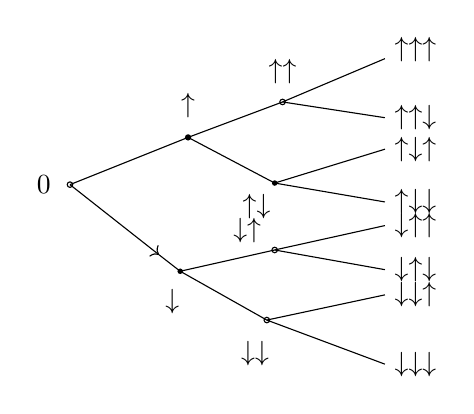
\begin{tikzpicture}[x=1cm,y=1cm]
\draw (0,0)--(1.5,0.6)--(2.7,1.05)--(4,1.6);
\draw (2.7,1.05)--(4,0.85);
\draw (1.5,0.6)--(2.6,0.02)--(4,0.45);
\draw (2.6,0.02)--(4,-0.22);
\draw[->] (0,0)--(1.13,-0.89);
\draw (1.13,-0.89)--(1.4,-1.1)--(2.6,-0.83)--(4,-0.52);
\draw (2.6,-0.83)--(4,-1.08);
\draw (1.4,-1.1)--(2.5,-1.72)--(4,-1.4);
\draw (2.5,-1.72)--(4,-2.28);
\draw (0,0) circle (0.035);
\fill (1.5,0.6) circle (0.04);
\draw (2.7,1.05) circle (0.035);
\fill (2.6,0.02) circle (0.035);
\fill (1.4,-1.1) circle (0.035);
\draw (2.6,-0.83) circle (0.035);
\draw (2.5,-1.72) circle (0.035);
\node[left] at (-0.12,0) {$0$};
\node[above] at (1.5,0.72) {$\uparrow$};
\node[above] at (2.7,1.15) {$\uparrow\uparrow$};
\node[below] at (2.37,0) {$\uparrow\downarrow$};
\node[below] at (1.3,-1.2) {$\downarrow$};
\node[above] at (2.25,-0.86) {$\downarrow\uparrow$};
\node[below] at (2.35,-1.87) {$\downarrow\downarrow$};
\node[right] at (4,1.72) {$\uparrow\uparrow\uparrow$};
\node[right] at (4,0.85) {$\uparrow\uparrow\downarrow$};
\node[right] at (4,0.45) {$\uparrow\downarrow\uparrow$};
\node[right] at (4,-0.22) {$\uparrow\downarrow\downarrow$};
\node[right] at (4,-0.52) {$\downarrow\uparrow\uparrow$};
\node[right] at (4,-1.08) {$\downarrow\uparrow\downarrow$};
\node[right] at (4,-1.4) {$\downarrow\downarrow\uparrow$};
\node[right] at (4,-2.28) {$\downarrow\downarrow\downarrow$};
\end{tikzpicture}
\end{adjustbox}
\end{center}

\Incomplete{GELFAND-P000786}{faint-formula-right}{Под числовой прямой, справа от дерева, сохранились фрагменты очень слабой формулы; различимы правая фигурная скобка и знак равенства, остальные знаки не читаются.}

\begin{equation*}
x\underset{\substack{\vert\\\text{earlier}\\\text{(раньше)}}}{\longleftarrow}y
\end{equation*}
(т. е. $x$ на пути от $0$ к $y$)

$y]$ — элемент мн-ва чисел, идущих раньше $y$

\underline{Опер. усечения} — $x$ из меньшего числа стрелок

$y\rceil$ число раньше $y$, но больше его

$y\rfloor$ —\,``\,— и меньше его

$x<y$ определено тоже

\begin{gather*}
\{y]\}=\{y\rfloor\}\cup\{y\rceil\},\\
\{y\rceil\}\cap\{y\rfloor\}=\Lambda
\end{gather*}

\underline{Пример:}

\underline{Основное опр.:}

\SourcePage{GELFAND-P000787}{unlabelled}
\underline{Теор. 1}

(простая)

$A,B$ — \underline{мн-ва чисел}

$\forall a\in A,b\in B$;
[зачёркнуто: \Unclear{GELFAND-P000787}{theorem-one-cancellation}{неразборчивый знак}]
$a<b$

\underline{Тогда} $\exists x:\quad a<x<b$.

\underline{и сущ. единств. самое раннее $x$.}

\underline{Доказ-во:} трансфин. инд., смотрим $x=0$ и если не смогли найти $x$
до нек-рого места, то смотрим дальше.

\underline{Обозначение:}

$\{A:B\}$ [зачёркнуто:
\Unclear{GELFAND-P000787}{notation-cancellation}{и?}]
или $\{a:b\}$

[Под скобкой:] скобки с петлёй

\underline{Сложение.}

с пом. трансфин. индукции.

\underline{Теорема 2}
\begin{equation*}
x=\{x\rfloor:x\rceil\}
\end{equation*}
(очевидно)

\underline{Опр. сложения.}
\begin{equation*}
x+y=\{x\rfloor+y,\ x+y\rfloor:\ x\rceil+y,\ x+y\rceil\}
\end{equation*}

\underline{Теорема 3.}

а) $0+0=\{:\}=0$.

[Под формулой:] нет условий, значит вообще самое раннее

б) [зачёркнуто:
\Unclear{GELFAND-P000787}{zero-quantifier-cancellation}{$\forall x$?}]
$x+0=x$ по индукции

\underline{Д-во:}
\begin{equation*}
x+0=\{x\rfloor+0:x\rceil+0\}
\underset{\text{инд.}}{=}
\{x\rfloor:x\rceil\}=x
\end{equation*}
[К последнему равенству направлена стрелка с подписью:] Теор. 2.

В обычн. теории нет понятия раньше!

$x+y$ — простейшее число, монот. по каждому аргументу

а) монот. по $x,y$

б) среди всех таких самое раннее.

Вып. обычные св-ва

\begin{equation*}
x+y=y+x
\end{equation*}

\Unclear{GELFAND-P000787}{associativity-sign}{$(x+y)+z=x+(y\ge z)$ / $(x+y)+z=x+(y+z)$}

\underline{Есть обр. операция.}

Противоп. к $x$ — обращ. стрелок
\qquad $x+\operatorname{opp}.x=0$.

\SourcePage{GELFAND-P000788}{5}
\Unclear{GELFAND-P000788}{top-sum}{$\uparrow+\uparrow=\{1,1:\Lambda\}=\uparrow\uparrow$ / $1+1=\{1,1:\Lambda\}=\uparrow\uparrow$}

\underline{\underline{Упр.}}
\begin{gather*}
\uparrow\downarrow+\uparrow\downarrow=?\\
\widehat{\uparrow}+\downarrow\downarrow\downarrow=?
\end{gather*}

\underline{Умножение.}

\underline{Basic inequality} of \underline{mult'n.}

\Unclear{GELFAND-P000788}{basic-letter}{$r$ / $\eta$}$<s,\quad u<v$.

Тогда

\Unclear{GELFAND-P000788}{basic-products}{$ru+sv>rv+su$?}

$xy$ — любое из 4-х \Unclear{GELFAND-P000788}{four-products-word}{слаг.? / оп.?}
$\Rightarrow$ 4 нер-ва

\begin{equation*}
\begin{aligned}
x\cdot y=\{&x\rfloor\cdot y+x\cdot y\rfloor-x\rfloor\cdot y\rfloor,\\
&x\rceil\cdot y+x\cdot y\rceil-x\rceil\cdot y\rceil:\\
&x\rfloor\cdot y+x\cdot y\rceil-x\rfloor\cdot y\rceil,\\
&x\rceil\cdot y+x\cdot y\rfloor-x\rceil\cdot y\rfloor\}
\end{aligned}
\end{equation*}
[У конца третьей строки, над запятой:]
\Unclear{GELFAND-P000788}{recursion-mark}{густой крестообразный знак; звёздочка или зачёркивание?}

Вып. естеств. св-ва умножения.

\begin{equation*}
x\cdot0=\{:\}=0,\qquad x\cdot1=x
\end{equation*}

\begin{equation*}
\begin{aligned}
x\cdot1&=\{x\rfloor\cdot1+x\cdot0-x\rfloor\cdot0:\\
&\qquad x\rceil\cdot1+x\cdot0-x\rceil\cdot0\}\\
&=\{x\rfloor+0-0:x\rceil+0-0\}=x
\end{aligned}
\end{equation*}

Ассоциат., коммут., дистрибу. есть.

[Волнисто подчёркнуто:] Доказать дома.

\underline{\underline{Совет.}} Технич. приём.

Док., что опред.
[зачёркнуто: \Incomplete{GELFAND-P000788}{advice-cancellation}{Сокращение густо зачёркнуто; возможно «умн.», уверенно прочитать не удалось.}]
[вписано над строкой со знаком вставки:] сложения
„нечувствит. к скобкам“

[Ниже, волнисто подчёркнуто:] bracket indifferent

\begin{gather*}
x=\{a:b\}\\
y=\{c:d\}\\
x+y=\{a+y,x+c:b+y,x+d\}
\end{gather*}

Умножение тоже обл. этим св-вом.

[Волнисто подчёркнуто:] Ассоциат.

Сущ. беск. большие и беск. малые числа.

\SourcePage{GELFAND-P000789}{unlabelled}
\begin{gather*}
\uparrow\uparrow\uparrow\ldots=\widehat{\uparrow}=\omega
\quad\text{— простейшее }\Unclear{GELFAND-P000789}{top-infinite-abbreviation}{\text{беск.}}\ \text{число.}\\
\uparrow\downarrow\downarrow\ldots=\uparrow\widehat{\downarrow}=\varepsilon
\end{gather*}

\begin{adjustbox}{max width=\linewidth}
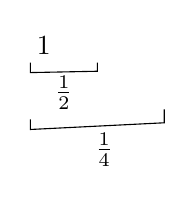
\begin{tikzpicture}[scale=0.85]
\draw (0,1.1)--(0,0.95)--(1,0.97)--(1,1.1);
\draw (0,0.25)--(0,0.1)--(2,0.2)--(2,0.4);
\node at (0.2,1.35) {$1$};
\node at (0.5,0.65) {$\frac12$};
\node at (1.1,-0.2) {$\frac14$};
\end{tikzpicture}
\end{adjustbox}

\begin{gather*}
\omega\cdot\varepsilon=1\\
\omega+\varepsilon=\widehat{\uparrow}\uparrow\widehat{\downarrow}
\end{gather*}
Иногда можно сократить, но не всегда.

\underline{Арифметика ординалов.}

[Зачеркнуто: \Incomplete{GELFAND-P000789}{ordinals-cancellation}{Слово под вставкой «ординалы» закрыто многократным зачеркиванием; полностью прочитать его не удалось.} Сверху вставлено: ординалы]: числа со стрелками $\uparrow$ (без стрелок $\downarrow$).

Арифметика — не обычная!

Обычная не коммутативна!

\begin{adjustbox}{max width=\linewidth}
\begin{tikzpicture}
\node at (0,0) {$\omega=$};
\node at (0.7,0) {$1$};
\node at (1.1,0) {$\oplus$};
\node at (1.55,0) {$\omega$};
\node at (2.1,0) {$\ne$};
\node at (2.65,0) {$\omega$};
\node at (3.1,0) {$\oplus$};
\node at (3.55,0) {$1$};
\node at (6.1,0) {Это её дефект};
\draw (1.1,-0.3)--(1.5,-0.9);
\draw (3.1,-0.3)--(2.85,-0.75);
\node at (2.1,-1.05) {обычная};
\node at (2.1,-1.4) {теория};
\end{tikzpicture}
\end{adjustbox}

\Unclear{GELFAND-P000789}{hessenburg-spelling}{Hessenburg}
\Unclear{GELFAND-P000789}{hessenburg-definition-abbreviation}{прид.}
естеств. опр. слож. и умн. трансфин. чисел.
Оказалось, что оно совпад. с этим

$\forall$ число, кроме $0$, имеет обратное $\frac1x$, $x\ne0$.

$\frac yx$ есть

\underline{$\forall\Unclear{GELFAND-P000789}{sqrt-overwritten-variable}{x}>0$ есть $\sqrt{x}$}
— \Unclear{GELFAND-P000789}{sqrt-proof-abbreviation}{по инд. беск.}

$\forall$ многочлен, \Unclear{GELFAND-P000789}{polynomial-abbreviation}{прин.} в $2^{\text{х}}$ точках знач. разных знаков, где-то между ними обр. в $0$; но это беск. без непр. — имеет щели, напр., между конеч. и беск. числами.

[Слева зачеркнут знак: \Unclear{GELFAND-P000789}{lower-cancelled-symbol}{неразборчиво}.]
$\Unclear{GELFAND-P000789}{largest-number-superscript}{\uparrow^{\ell}}$ — «самое большое» $\longrightarrow$ [над «не» вставлено: уже] не сюрреал. число.

\begin{gather*}
\widehat{\uparrow\downarrow}=\frac23
\qquad \uparrow\downarrow\uparrow=\frac34\\
\widehat{\uparrow}\Unclear{GELFAND-P000789}{gap-superscript}{\downarrow^{\ell}}
\quad\text{— дыра}
\end{gather*}

есть $\exp x$; $x^y$; $\log$

\SourcePage{GELFAND-P000790}{6}
Если $x$ — полож. беск., то
\begin{equation*}
2^x>x^n\qquad\text{для любого }n.
\end{equation*}
$x$ — беск. малое $\Rightarrow$
\begin{equation*}
\exp x=\sum_{n\in\text{кон.}}\frac{x^n}{n!}
\end{equation*}
$x$ — беск. малое, $n$ — вещ. $\Rightarrow$ ряд $\sum x^n a_n$ сход. $\forall a_n$

Одно из возм. прил. теории:
\begin{equation*}
\int_x^{\Unclear{GELFAND-P000790}{integral-upper-limit}{\uparrow^{\ell}}}e^{-\xi^2}\,d\xi
=\sum\frac{n!}{x^n}
\end{equation*}

Всякое число $=$ отнош. 2-х целых чисел $\left(=\frac mn\right)$.

\begin{equation*}
\widehat{\uparrow}\downarrow=\omega-1
\end{equation*}
\begin{equation*}
|x]-x|=1\qquad\text{— опр. целого числа}
\end{equation*}

\begin{gather*}
\exp x=\\
=\{0,\ \exp x]\cdot\sum_{m=1}^{n}\frac{(x-x]^{m}}{m!}
:\ \exp x]\big/\sum_{m=0}^{n}\frac{(x]-x)^m}{m!}
\end{gather*}
\Unclear{GELFAND-P000790}{exponential-delimiters}{В первой сумме после правой квадратной скобки закрывающая круглая скобка не различима; заключительная фигурная скобка формулы не написана.}

\SourcePage{GELFAND-P000791}{unlabelled}
\underline{13.11.78.}\qquad\underline{Сем. Гельфанда}

\underline{А. Поляков}\qquad\underline{2-мерная дискр. система.}

\begin{equation*}
(1)\qquad S=\operatorname{Tr}\sum_{\vec{x},\vec{\delta}}g_{\vec{x}}^{-1}g_{\vec{x}+\vec{\delta}}
\end{equation*}

\begin{adjustbox}{max width=\linewidth}
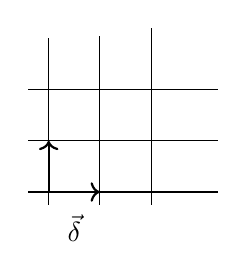
\begin{tikzpicture}[scale=0.65]
\draw (-0.4,0)--(3.3,0);
\draw (-0.4,1)--(3.3,1);
\draw (-0.4,2)--(3.3,2);
\draw (0,-0.25)--(0,3);
\draw (1,-0.25)--(1,3.05);
\draw (2,-0.25)--(2,3.2);
\draw[->,thick] (0,0)--(1,0);
\draw[->,thick] (0,0)--(0,1);
\node at (0.5,-0.7) {$\vec{\delta}$};
\end{tikzpicture}
\end{adjustbox}

\begin{gather*}
(2)\qquad g_{\vec{x}}\in GL(n,R)\\
(3)\qquad \partial_\mu F_{\mu\nu}(x)+[A_\mu,F_{\mu\nu}]=0\\
(4)\qquad \sum_\delta\left\{\underbrace{g_{\vec{x}+\vec{\delta}}g_{\vec{x}}^{-1}}_{A_{\vec{x}\delta}}-g_{\vec{x}}g_{\vec{x}-\vec{\delta}}^{-1}\right\}=0
\end{gather*}

\underline{Сист. вполне интегр.} и есть беск. набор токов.
(есть $L,A$-пара и \Unclear{GELFAND-P000791}{integrability-note-end}{т.?})
[Под словом «есть» вписано: интегралы.]

\begin{equation*}
(5)\qquad\sum_\delta\left(J_{\vec{x}\delta}^{(k)}-J_{\vec{x}-\vec{\delta},\delta}^{(k)}\right)=0
\end{equation*}

\underline{Примеры токов:}
\begin{gather*}
(6)_1\qquad J_{\bar{x}\delta}^{(1)}=A_{x\delta}\\
(6)_2\qquad J_{\bar{x}\delta}^{(2)}=\varepsilon_{\delta\gamma}A_{\bar{x}\gamma}+
\end{gather*}
\Unclear{GELFAND-P000791}{current-indices}{Короткие надчеркивания над $x$ в формулах $(6)_1$, $(6)_2$ переданы как черты; стрелочные концы не различимы.}
\Unclear{GELFAND-P000791}{current-j2-ending}{Формула $(6)_2$ заканчивается знаком $+$; дальнейшее слагаемое не записано.}

Для аб. группы и в пределе (непр.) по одной пер. — цепочка Тода.

Здесь дискр. время. и неаб. случай

Цеп. Тода:
\begin{equation*}
(7)\qquad \mathcal{L}=\operatorname{Tr}\sum_s\left(\Unclear{GELFAND-P000791}{kinetic-first-factor}{\dot{g}_s^{-1}}\dot{g}_s+g_s^{-1}g_{s+1}\right)
\end{equation*}
Положим
\begin{equation*}
(8)\qquad\begin{cases}
A_s=g_s^{-1}\dot{g}_s\\
B_s=g_s^{-1}g_{s+1}
\end{cases}
\end{equation*}

Условия нулевой кривизны:
\begin{equation*}
(9)\qquad\begin{cases}
\dot{B}_s+A_sB_s-B_sA_{s+1}=0\\
\dot{A}_s=B_s-B_{s-1}
\end{cases}
\end{equation*}
[Справа от первой строки: (усл. [зачеркнуто: \Unclear{GELFAND-P000791}{zero-curvature-cancellation}{связности?}]); ниже вписано: 0-й кривизны.]

Найдём $L_s$, $M_s$, тоже уд. условию 0-й крив.
\begin{equation*}
(10)\qquad\dot{L}_s\Unclear{GELFAND-P000791}{lax-overwritten-sign}{+}M_sL_s-L_sM_{s+1}=0
\end{equation*}
Хотим:
\begin{equation*}
L_s(A,B,\lambda),\ M_s(A,B,\lambda)
\end{equation*}
так что $(10)\Rightarrow(9)$ и наоборот.

Тогда

\SourcePage{GELFAND-P000792}{17}

\begin{equation}
\frac{d}{dt}\left\{\prod_{s=-\infty}^{\infty}L_s\right\}=0
\tag{11}
\end{equation}

\Unclear{GELFAND-P000792}{top-isolated-stroke}{[Под произведением отдельный короткий штрих с точкой, похожий на $i$.]}

произв. ф-я всех интегралов

\begin{center}
\begin{adjustbox}{max width=\linewidth}
\begin{tikzpicture}[x=1cm,y=1cm]
\draw[->] (-1.3,0) -- (2.2,0) node[right] {$s$};
\draw[->] (0,-0.6) -- (0,1.35) node[right] {$t$};
\draw (1.4,0.18) -- (1.4,0.72) -- (-1.3,0.72);
\draw[->] (-1.3,0.68) -- (-1.3,0.02);
\end{tikzpicture}
\end{adjustbox}
\end{center}

$L,M$ — связности

\begin{equation*}
I(0)\underset{\mathrm{def}}{=}\prod L_s(0)
\end{equation*}

Т. к.
\begin{equation*}
I(0)I^{-1}(\delta t)=1,
\end{equation*}
то $I(\delta t)=I(0)$ и $I(t)$ — интеграл дв-ния.

„Тупой способ“ поиска $L,A$-пары: итерации по $\lambda$

\underline{ответ.}

\begin{equation}
L_s=1+\lambda A_s-\lambda^2B_sL_{s+1}^{-1}
\tag{12}
\end{equation}

Итерир. по $\lambda$

\begin{equation*}
\prod_s(1+\lambda A_s)
\Unclear{GELFAND-P000792}{product-expansions}{=}
1+\lambda\left(\sum A_s\right)
\end{equation*}

\begin{equation}
\prod(1+\lambda A_s-\lambda^2B_s)
\Unclear{GELFAND-P000792}{product-expansions}{=}
1+\lambda\sum A_s+\lambda^2
\begin{adjustbox}{max width=\linewidth}
\begin{tikzpicture}[baseline=0,x=1cm,y=1cm]
\node[anchor=base west,inner sep=0] at (0,0) {$\displaystyle\left(\sum_{s<s'}A_sA_{s'}-\sum B_s\right)$};
\draw (0,-0.58) -- (0,-0.74) -- (5.6,-0.74) -- (5.6,-0.58);
\node at (2.8,-1.07) {нетрив. интеграл};
\draw (1.08,-1.35) .. controls (1.36,-1.19) and (1.48,-1.51) .. (1.79,-1.35) .. controls (2.13,-1.23) and (2.28,-1.47) .. (2.62,-1.35) .. controls (2.96,-1.23) and (3.15,-1.47) .. (3.49,-1.35) .. controls (3.8,-1.23) and (4.04,-1.47) .. (4.39,-1.35);
\end{tikzpicture}
\end{adjustbox}
\tag{13}
\end{equation}

\begin{equation}
\begin{cases}
L_s=e^{-\partial}+A_s+B_se^{\partial}\\
\text{[зачёркнуто]}\qquad M_s=B_se^{\partial}
\end{cases}
\tag{14}
\end{equation}

[В начале второй строки (14) зачёркнуто:
\Incomplete{GELFAND-P000792}{equation-14-cancellation}{Выражение закрыто густой штриховкой; его исходные знаки не читаются.}]

Здесь $e^{\partial}$ — смещ. на 1 на решётке

$L_s,M_s$ — разностные операторы (Матр. Якоби)

\underline{Калибровочная теория.}

\begin{center}
\begin{adjustbox}{max width=\linewidth}
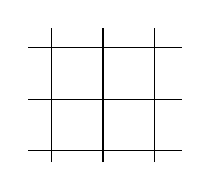
\begin{tikzpicture}[x=1cm,y=1cm,baseline=0]
\draw (-0.3,0) -- (1.65,0);
\draw (-0.3,0.65) -- (1.65,0.65);
\draw (-0.3,1.3) -- (1.65,1.3);
\draw (0,-0.15) -- (0,1.55);
\draw (0.65,-0.15) -- (0.65,1.55);
\draw (1.3,-0.15) -- (1.3,1.55);
\end{tikzpicture}
\end{adjustbox}
\qquad $B_{\vec{x}\alpha}$
\end{center}

$\vec{x}$ — точка, $\alpha$ — направление

($\alpha=1,\ldots,d$ —\newline
— $d$ — размерность)

2-мерн. случай — 2 напр.

(берутся только положительные)

\SourcePage{GELFAND-P000793}{unlabelled}

\begin{equation}
F_{\bar{x}\alpha\beta}=
B_{\bar{x},\alpha}
B_{\bar{x}+\bar{\alpha},\beta}
B^{-1}_{\bar{x}+\bar{\beta},\alpha}
B^{-1}_{\bar{x},\beta}
\tag{15}
\end{equation}

Действие:
\begin{equation}
S=\sum_{\bar{x},\alpha,\beta}\mathrm{Tr}\,F_{\vec{x}\alpha\beta}
\tag{16}
\end{equation}

[Справа:] Классич. пред. $\longrightarrow$
$\Unclear{GELFAND-P000793}{action-classical-square}{F^2}$

($e^f\Unclear{GELFAND-P000793}{action-exponential}{=}1+f+\frac{f^2}{2}$
[под $f$, с соединяющим штрихом: лин. член сокр.])

\underline{Ур-я движения:}
[Подчёркнуто волнистой линией.]

\begin{equation}
\sum\left\{
\begin{adjustbox}{max width=\linewidth}
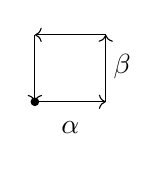
\begin{tikzpicture}[baseline=0,x=1cm,y=1cm]
\draw[->] (0,0.35) -- (0.9,0.35);
\draw[->] (0.9,0.35) -- (0.9,1.2);
\draw[->] (0.9,1.2) -- (0,1.2);
\draw[->] (0,1.2) -- (0,0.35);
\fill (0,0.35) circle (0.055);
\node at (0.45,0.02) {$\alpha$};
\node at (1.11,0.8) {$\beta$};
\end{tikzpicture}
\end{adjustbox}
-
\begin{adjustbox}{max width=\linewidth}
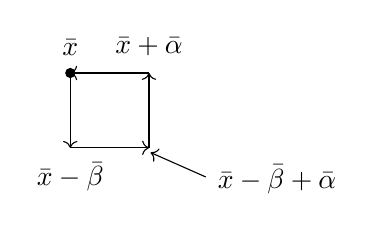
\begin{tikzpicture}[baseline=0,x=1cm,y=1cm]
\draw[->] (1,0) -- (0,0);
\draw[->] (0,0) -- (0,-0.95);
\draw[->] (0,-0.95) -- (1,-0.95);
\draw[->] (1,-0.95) -- (1,0);
\fill (0,0) circle (0.065);
\node[above] at (0,0.1) {$\bar{x}$};
\node[above] at (1,0.1) {$\bar{x}+\bar{\alpha}$};
\node[below] at (0,-1.01) {$\bar{x}-\bar{\beta}$};
\node[right] at (1.75,-1.35) {$\bar{x}-\bar{\beta}+\bar{\alpha}$};
\draw[->] (1.72,-1.32) -- (1.02,-1.01);
\end{tikzpicture}
\end{adjustbox}
\right\}=0
\tag{17}
\end{equation}

Точкой выделено начало

$\sum_\beta$, $\alpha$ — фиксир.
\qquad (Ср.:
$\Unclear{GELFAND-P000793}{motion-comparison-operator}{\nabla}_{\beta}F_{\alpha\beta}=0$)

В 2-\Unclear{GELFAND-P000793}{dimension-overwriting}{мерн.} случае нет суммир.

(17) означает:

\begin{equation*}
\begin{aligned}
(17)_2\quad\sum\bigl\{&
B_{\bar{x},\alpha}
B_{\bar{x}+\bar{\alpha},\beta}
B^{-1}_{\bar{x}+\bar{\beta},\alpha}
B^{-1}_{\bar{x},\beta}
-B^{-1}_{\Unclear{GELFAND-P000793}{motion-expanded-first-inverse}{\bar{x},\beta}}
B_{\bar{x}-\bar{\beta},\alpha}
B_{\bar{x}-\bar{\beta}+\bar{\alpha},\beta}
B^{-1}_{\bar{x}\alpha}
\bigr\}=0
\end{aligned}
\end{equation*}

\begin{equation}
\Psi\left(\Unclear{GELFAND-P000793}{contour-18-argument}{c_{\bar{y}}}\right)=
\begin{adjustbox}{max width=\linewidth}
\begin{tikzpicture}[baseline=0,x=1em,y=1em]
\node[anchor=base,inner sep=0] at (0,0) {$\displaystyle\prod$};
\draw (0,0.34) ellipse (0.65 and 0.3);
\node at (0,-1.25) {$\Unclear{GELFAND-P000793}{contour-18-product-subscript}{C_{\bar{y}}}$};
\end{tikzpicture}
\end{adjustbox}
B_{\Unclear{GELFAND-P000793}{contour-18-b-subscript}{\bar{x}}\beta}
\qquad
\begin{adjustbox}{max width=\linewidth}
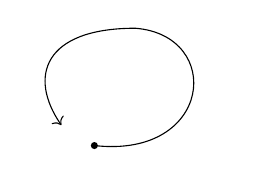
\begin{tikzpicture}[baseline=0,x=1cm,y=1cm]
\fill (0,-0.45) circle (0.045);
\draw[->] (0,-0.45) .. controls (1.5,-0.62) and (1.65,0.95) .. (0.52,1.04) .. controls (-0.65,1.04) and (-0.84,0.42) .. (-0.42,-0.19);
\end{tikzpicture}
\end{adjustbox}
\tag{18}
\end{equation}

Рассм.
\begin{equation*}
\Psi(c_y+\Pi_{\bar{x}\alpha\beta})
\end{equation*}

\begin{equation*}
C+\Pi_{\bar{x}\alpha\beta}=
\begin{adjustbox}{max width=\linewidth}
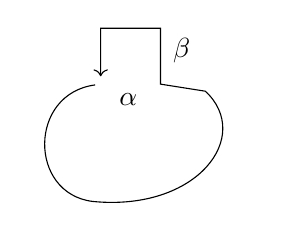
\begin{tikzpicture}[baseline=0,x=1cm,y=1cm]
\draw[->] (-0.45,-0.07) .. controls (-1.3,-0.18) and (-1.3,-1.45) .. (-0.48,-1.55) .. controls (0.85,-1.68) and (1.56,-0.72) .. (0.95,-0.15) -- (0.38,-0.06) -- (0.38,0.65) -- (-0.38,0.65) -- (-0.38,0.04);
\node at (-0.03,-0.26) {$\alpha$};
\node at (0.65,0.37) {$\beta$};
\end{tikzpicture}
\end{adjustbox}
\end{equation*}

приклеили мал. квадратик

Теперь

\begin{equation}
\Psi\left(\Unclear{GELFAND-P000793}{contour-19-case}{c}+
\Pi_{\bar{x}\Unclear{GELFAND-P000793}{contour-19-alpha}{\alpha}\beta}\right)
\Psi^{-1}(C)=
\tag{19}
\end{equation}

\SourceFigure{GELFAND-P000793}{transport-19-diagram}{Слева вверху небольшой почти прямоугольный контур; у его нижнего правого угла начинаются две близкие дуги, изгибающиеся вправо и вниз. Внизу они сходятся возле малой петли; под этим местом написано $y$. Нижняя горизонталь прямоугольника имеет тёмный след возле левого конца. Точные соединения и направления стрелок в местах разрывов неуверенны.}

напр. в т. $\bar{x},\alpha$, перенес.
в точку $y$

Ур-я запис. в виде:

\begin{equation}
\sum_\beta\left\{
\Psi\left(\Unclear{GELFAND-P000793}{contour-20-case}{c}+
\Pi_{\bar{x}\Unclear{GELFAND-P000793}{contour-20-overwritten-indices}{\alpha\beta}}\right)
\Psi^{-1}(C)-\Psi(C)\Psi^{-1}(C-\Pi_{\bar{x}\alpha\beta})
\right\}=0
\tag{20}
\end{equation}

Получ. что-то вроде связности (тривиальной) в пр-ве контуров.

(т. е. [над строкой вставлено: матр.] функция контура)

(ср. с (4))

\underline{Непр. случай.}
[Подчёркнуто волнистой линией.]

$\Psi[x_{\Unclear{GELFAND-P000793}{continuous-overwritten-index}{\mu}}(s)]$ — функционал от кривой

(не зав. от параметризации)

[Справа:] $x(s)=(x_\mu(s));$

$\mu=1,2,3,4.$

Ток
\begin{equation}
\mathcal{F}_\mu(s,C)=\frac{\delta\Psi(x(s))}{\delta x_\mu(s)}\Psi^{-1}
\tag{21}
\end{equation}

\SourcePage{GELFAND-P000794}{18}

\underline{\underline{Ур-е:}}

\begin{equation*}
(22)_1\qquad
\frac{\delta\mathcal{F}_\mu(s,C)}{\delta x_\mu(s)}=0
\end{equation*}

[Справа, объединено скобкой:]
\begin{quote}
$\Psi$ прин. знач. в группе,\newline
а $\mathcal{F}$ — в алгебре Ли
\end{quote}

$\Psi$ Инв. отн. параметризации: это запис. в виде
\begin{equation*}
(23)\qquad
\frac{dx_\mu}{ds}\frac{\delta\Psi}{\delta x_\mu(s)}=0
\end{equation*}

\begin{gather*}
\mathcal{F}_\beta=\Psi(c+\Pi_{\alpha\beta})\Psi^{-1}(c)
\\
\sum_\beta\{\mathcal{F}_\beta(c)-\mathcal{F}_\beta(c-\Pi_{\alpha\beta})\}=0
\end{gather*}
\Unclear{GELFAND-P000794}{discrete-contour-case}{Регистр буквы $c$ в этих двух строках не вполне различим.}

непр. предел дает (22).

\begin{equation*}
\Psi=p\,e^{\oint A_\mu\,dx_\mu}
\end{equation*}

\begin{equation*}
(22)_2\qquad
\frac{\delta\mathcal{F}_\mu(s)}{\delta x_\nu(s')}
-\frac{\delta\mathcal{F}_\nu(s')}{\delta x_\mu(s)}
+[\mathcal{F}_\mu(s),\mathcal{F}_\nu(s')]=0
\end{equation*}
[В номере вторая цифра переписана: \Unclear{GELFAND-P000794}{equation-22b-number}{2; первоначальная цифра неясна}.]

Действие
\begin{equation*}
\text{\Unclear{GELFAND-P000794}{action-number}{(24) / (21)}}\qquad
S=\int\left(\frac{\delta\Psi^{-1}}{\delta x_\mu(s)}
\frac{\delta\Psi}{\delta x_\mu(s)}\right)(Dx_\mu(s))
\end{equation*}
Неясно, как определять

\underline{Аккуратно:} 3 измерения.

(в $4^{\text{х}}$ ещё не до конца проверено).

Решаются ур-я $(22)_1$ — $(22)_2$, где $\mathcal{F}$ получ. по ф-ле (21),
а $\Psi$ удовл. усл. (23).

Поле Я.-М. — киральное поле на пр-ве петель.

На петлях — ф-я со знач. в конечномерной группе; для него ур-я
главного кир. поля ($\Psi$ — такое поле) — (22).

[Слева над строкой вписано: Если.]
$\Psi$ \underline{из связности}
($\Leftrightarrow$ $\Psi$ — гомом. петель в группу) $\Rightarrow$
получ. ур-я Я.-Миллса.

\underline{Токи:} ($\sim$ интегралы дв-ния):
\begin{equation*}
(25)\qquad
\frac{\delta\mathcal{J}^{(k)}_\mu(s,C)}{\delta x_\mu(s)}=0
\end{equation*}

\SourcePage{GELFAND-P000795}{unlabelled}

\begin{equation*}
(26)\qquad \mathcal{J}^{(1)}_\mu=\mathcal{F}_\mu(s,C)
\end{equation*}

\begin{equation*}
(27)\qquad
\mathcal{J}^{(2)}_\mu=\varepsilon_{\mu\nu\lambda}\,t_\nu(s)\mathcal{F}_\lambda(s,C)
+[\mathcal{F}_\mu(s),\chi]
\end{equation*}

$t$ — касат. вектор к кривой

[Зачёркнут знак: \Unclear{GELFAND-P000795}{cancel-before-chi}{$\mathcal{F}$}.]
$\chi$ сейчас найдем

Имеем:
\begin{equation*}
(28)\qquad
\frac{\delta\Unclear{GELFAND-P000795}{derivative-current-glyph}{\mathcal{J}}^{(2)}_\mu}{\delta x_\mu}
=\underset{\substack{\Vert\\\displaystyle\varepsilon_{\mu\nu\lambda}t_\nu[\mathcal{F}_\mu,\mathcal{F}_\lambda]}}
{\varepsilon_{\mu\nu\lambda}\,t_\nu(s)\frac{\delta\mathcal{F}_\lambda(s,c)}{\delta x_\mu(s)}}
+\left[\mathcal{F}_\mu(s,c),\frac{\delta\chi}{\delta x_\mu(s)}\right]
\end{equation*}
\Unclear{GELFAND-P000795}{derivative-identity}{Коэффициент в равенстве под первым слагаемым требует проверки; запись сохранена.}

Пусть
\begin{equation*}
(29)\qquad
\frac{\delta\chi}{\delta x_\mu}=-\varepsilon_{\mu\nu\lambda}\,t_\nu\mathcal{F}_\lambda
\end{equation*}

Тогда
\begin{equation*}
(30)\qquad
\mathcal{F}_\mu=\varepsilon_{\mu\nu\lambda}\,t_\nu\frac{\delta\chi}{\delta x_\lambda}
\end{equation*}

Это возможно при вып. $(22)_1$

Получ. нелокальный закон сохранения.
\Unclear{GELFAND-P000795}{figure-intro}{Выраж-е.} $\chi$:

\SourceFigure{GELFAND-P000795}{loop-tail-expansion}{Запись $\chi=$, затем четыре петли, разделённые знаками $+$, после четвёртой — $+\ldots$. Первая петля овальная, без выступа; у следующих трёх сверху узкие прямоугольные выступы возрастающей длины. В последнем выступе несколько утолщённых и повторных штрихов; принадлежность этих штрихов стрелкам и их направления не вполне различимы.}

(пристраивается хвост по одному направлению)

Нелокальность 1-мерная.

\underline{Контура:} 1. S. Mandelstam, Phys. Rev., 1968.

2. Минлос, Синай

[Справа, на высоте пункта 1:]
квант. Я.-М. в духе Фаддеева-Попова

\underline{\Unclear{GELFAND-P000795}{pencil-heading-sign}{$\gamma$ / $\lambda$}-пучок}
(вместо $L,A$-пары)

\begin{equation*}
(31)\qquad
\frac{\delta\varphi}{\delta x_\mu(s)}
+\text{\Unclear{GELFAND-P000795}{equation-31-parameter}{z / Z}}\,
\varepsilon_{\mu\nu\lambda}\,t_\nu\frac{\delta\varphi}{\delta x_\lambda}
=\mathcal{F}_\mu(s,C)\varphi(s,C)
\end{equation*}

\Unclear{GELFAND-P000795}{parameter-note}{z / Z} — произв. параметр

Аналог. вид имеет:

\underline{Станд. киральное поле} (Pohlmayer, Захаров, Михайлов):
\begin{equation*}
(32)\qquad
A_\mu=g^{-1}\partial_\mu g(x);\qquad
\left[\partial_\mu+
\text{\Unclear{GELFAND-P000795}{equation-32-parameter}{z / Z}}\,
\varepsilon_{\mu\nu}\partial_\nu\right]\varphi=A_\mu\varphi,
\qquad\mu=1,2,\,..
\end{equation*}
\SourcePage{GELFAND-P000796}{19}
(31) — система ур-й, $z$ — спектр. параметр.

Совместность (31) $\Rightarrow$ ур-я (22).
\begin{equation*}
z=0\quad\Rightarrow\quad\varphi=\Psi
\end{equation*}
\underline{Интегралы} — ?

На модели (32) посмотрим, как получ. интегралы.
\begin{equation*}
(32)\Leftrightarrow
\end{equation*}
\begin{equation*}
\partial_\mu\varphi=\frac{A_\mu+z\varepsilon_{\mu\nu}A_\nu}{1-z^2}\,\varphi
\tag{33}
\end{equation*}
\begin{equation*}
P\exp\oint_C\frac{A_\mu+z\varepsilon_{\mu\nu}A_\nu}{1-z^2}\,dx^\mu=1
\tag{34}
\end{equation*}
(упор. экспон)

Спец. выбор контур:
\SourceFigure{GELFAND-P000796}{contour-01}{Справа от (34)–(35): контур $C$, узкий прямоугольник на пересечении горизонтальной и вертикальной осей. Верхняя стрелка направлена влево, левая — вниз, правая — вверх, нижняя справа — вправо; дополнительные штрихи у нижнего левого угла требуют проверки по оригиналу.}
\begin{equation*}
\frac{d}{dt}\,P\exp\int_{-\infty}^{\infty}dx_1
\left\{\frac{A_1+zA_2}{1-z^2}\right\}=0
\tag{35}
\end{equation*}
Это производ. \underline{ф-я интегралов} дв-ния.

Обычные соотн. переносятся в „контурологию“.

Есть диагр. Фейнмана, где вместо линий — поверхности.

Для своб. теории поля
\begin{adjustbox}{max width=\linewidth}
\begin{tikzpicture}[baseline=0pt]
\draw[->] (0,0) -- (1.8,0);
\fill (0,0) circle (0.025);
\node[below] at (0,0) {$x$};
\node[below right] at (1.8,0) {$x'$};
\end{tikzpicture}
\end{adjustbox}
ф-я Грина $G(x,x')$
удовл. ур-ю К.-Г.
\begin{equation*}
(\partial_x^2-m^2)G(x,x')=\delta(x-x')
\tag{36}
\end{equation*}
\begin{equation*}
G(x,x')\underset{|x-x'|\to\infty}{\sim}e^{-m|x-x'|}
\tag{37}
\end{equation*}
Здесь на контурах
\begin{equation*}
\left\{\frac{\delta^2}{\delta x_\mu^2(s)}-m^4\left(\frac{dx_\mu}{ds}\right)^2\right\}G(C)=0
\tag{38}
\end{equation*}
\begin{equation*}
G(C)=\langle\Psi(C)\rangle
\tag{39}
\end{equation*}
Как найти конт. ф-ю Грина?

\underline{Мат. задача:} (38) — „струнное“ ур-е К.-Г.

Гран. условие: убыв. при больших контурах:
\begin{equation*}
G(C)\sim e^{-m^2A(C)}
\tag{40}
\end{equation*}
($A(C)$ — мин. площадь, натян. на контур $C$)

\SourcePage{GELFAND-P000797}{unlabelled}
Пусть $G$ зав. лишь от тензоров
\begin{equation*}
\sigma_{\alpha\beta}=\oint_C x_\alpha\,dx_\beta
\tag{41}
\end{equation*}
\begin{equation*}
\frac{\delta\sigma_{\alpha\beta}}{\delta x_\mu(s)}
=\delta_{\alpha\mu}\frac{dx_\beta}{ds}
-\delta_{\beta\mu}\frac{dx_\alpha}{ds}
\tag{42}
\end{equation*}
\begin{equation*}
t_\mu(s)=\frac{dx_\mu}{ds}
\end{equation*}
[Перед $t_\alpha t_\beta$ зачеркнуто:
\Unclear{GELFAND-P000797}{eq43-cancel}{знак суммы с индексами или коэффициент; зачеркнутые знаки неразборчивы.}]
\begin{equation*}
t_\alpha t_\beta
\left[\frac{\partial^2}{\partial\sigma_{\alpha\gamma}\partial\sigma_{\beta\gamma}}
-m^4\delta_{\alpha\beta}\right]G=0
\tag{43}
\end{equation*}
Пусть
\begin{equation*}
\Pi_{\alpha\beta}=\frac{\partial}{\partial\sigma_{\alpha\beta}}
\end{equation*}
Тогда получаем
\begin{equation*}
\Pi_{\alpha\beta}\Pi_{\beta\gamma}=C\delta_{\alpha\beta};
\tag{44}
\end{equation*}
[После знака равенства, перед $C\delta_{\alpha\beta}$, зачеркнуто:
\Unclear{GELFAND-P000797}{eq44-cancel}{$\frac14\Pi^2_{\ldots}\delta_{\ldots}$; нижние индексы под зачёркиванием неразборчивы.}]
\Unclear{GELFAND-P000797}{eq44-indices}{В правой части (44) написано $\delta_{\alpha\beta}$.}

Это возм. лишь при
\begin{equation*}
\Pi_{\alpha\beta}=\pm{}^*\Pi_{\alpha\beta}
=\pm\varepsilon_{\alpha\beta\gamma\delta}\Pi_{\gamma\delta}
\tag{45}
\end{equation*}
Отсюда ф-я лишь от
\begin{equation*}
U_\pm=\sqrt{\sigma_{\alpha\beta}^2\pm\sigma_{\alpha\beta}\,{}^*\sigma_{\alpha\beta}}
\tag{46}
\end{equation*}
Явное решение:
\begin{equation*}
G(U_+,U_-)
\end{equation*}
выраж. через ф-и Бесселя.

[Между строками:] Смотрим на бесконечности:

Мин. площадь
\begin{equation*}
A_{\min}(C)=\sqrt{\sigma^2\pm\sigma\,{}^*\sigma}
\tag{47}
\end{equation*}
$\sigma$ — проекция на коорд. плоск.
\begin{equation*}
\sigma_{\alpha\beta}=\oint x_\alpha\,dx_\beta
\end{equation*}
\begin{equation*}
A=\int\sqrt{\dot{x}^{\,2}x'^{\,2}-(\dot{x}x')^2}\,dt\,ds
\end{equation*}
Ур-е Эйлера даёт
\begin{equation*}
A_{\min}(x(s))
\end{equation*}

\SourcePage{GELFAND-P000798}{20}
Ур-е Гам.-Якоби
\begin{equation*}
\left(\frac{\delta A_{\min}}{\delta x_\mu(s)}\right)^2
=\left(\frac{dx_\mu}{ds}\right)^2
\end{equation*}
Находим решение. (47) — удовл. ур-ю Гам.-Якоби.

Для не слишком [зачеркнуто:
\Unclear{GELFAND-P000798}{text-cancel}{неразборчивое короткое слово или начало слова.}]
перекруч. контуров (47) — решение.

Синай утв., что у Куранта что-то есть.

\SourcePage{GELFAND-P000799}{unlabelled}
\underline{\underline{20.11.78.}}\qquad\underline{\underline{Сем. Гельфанда.}}

«Торт с кофе не фокстрот»

«Сенсация: поп яйца снес»

[Справа:] «Я иду с мечем судия»

[Три записи объединены правой скобкой:] \underline{Палиндромы.}

\underline{Кричевер:} инстантоны без расслоений.

\underline{\underline{А. С. Шварц.}}

1. \underline{Квантовая} [вставлено над строкой: \underline{теор. поля и}]
\underline{статфиз.} — наука о вычислении интеграла (стат. суммы)
\begin{equation*}
Z=\int e^{-S(A)}\,dA
\tag{1}
\end{equation*}
$A$ пробегает пр-во траекторий или историй: \underline{$A=A(x,t)$}.

\underline{Смысл:} заменяем на конечномерный (сеточная аппрокс.) и переходим к пределу;
$a$ — [зачеркнуто: \Unclear{GELFAND-P000799}{step-cancel}{шаг?; зачеркнутое слово не установлено.}] шаг решётки.

\underline{КТП:} предел при $a\to0$ не сущ. (ультрафиолетовые расход.)

[Приписка под скобками; стрелка $\uparrow$ к предыдущей строке:]
решётка — обрез. по импульсам.

Один из выходов: переходить к пределу для коррелл. ф-й, т.е. вычислять
\begin{equation*}
\frac{\int\varphi(A)e^{-S(A)}\,dA}{\int e^{-S(A)}\,dA}
\tag{2}
\end{equation*}
(ф-и Грина или корреляц. ф-и).

\underline{Важно:} предел отношения уже имеет смысл.

\underline{Ещё:} при снятии обрезания надо делать „перенормировку“, т.е. входящ.
параметр $\lambda_a$ менять в зав. от $a$ при переходе к пределу.

\underline{Сущ. 2 метода вычисления конт. инт.:}

\underline{теория возмущ.} и \underline{квазиклассика}

(на самом деле 1-е — част. случай).

\underline{Важный класс функционалов} $S$, \underline{к-рый обл.}
\underline{\underline{вырождением}},

т.е. допускающим. $\infty$-мерную группу симметрии:
\begin{equation*}
g\in G\quad\leadsto\quad A\mapsto A^g
\end{equation*}
\begin{equation*}
\underline{S(A^g)=S(A)}
\tag{3}
\end{equation*}
\underline{Физические примеры:} калибровочные теории.

Чистая теория Я.-М.; $A=(A_\mu(x))$, $A_\mu\in$ алг. Ли конч. группы Ли.
\begin{equation*}
S(A)=\int\langle F_{\mu\nu},F^{\mu\nu}\rangle\,dV,
\tag{4}
\end{equation*}
где
\begin{equation*}
F_{\mu\nu}=\partial_\mu A_\nu-\partial_\nu A_\mu+[A_\mu,A_\nu]
\tag{5}
\end{equation*}

\SourcePage{GELFAND-P000800}{26}
\underline{Группа симметрии:}

если $g(x)$ — ф-я со знач. в группе Ли, то она порождает преобр. полей
\begin{equation*}
A_\mu\mapsto gA_\mu g^{-1}+g\partial_\mu(g^{-1})
\tag{6}
\end{equation*}
[Над следующей строкой зачеркнуто:
\Unclear{GELFAND-P000800}{upper-cancel}{неразборчивое короткое слово.}]

\underline{Способ борьбы с вырожд.: в случае эл-магн. поля:}

«Потенциалы не им. смысла», наложим калибр. условие
\begin{equation*}
\partial_\mu A_\mu=0
\tag{7}
\end{equation*}
\underline{Трудности:} трудно постр. теорию возмущений.

2. \underline{Квазиклассика} $\sim$ метод стац. фазы или Лапласа.

а) Давно реш. задача: как писать конт. интеграл (\underline{Фаддеев и Попов})

[Под строкой:] — на физ. уровне строгости.

б) Мат. теория — когда $S$ квадратичен.

в) Применение к вычисл. инстантонного вклада.

г) Инварианты Рэя-Зингера.

а) \underline{Квантование выр. лагранжианов.}

\underline{Трудность:} интеграл расходится, т.к. объём орбит бесконечен.

\underline{мораль:} выбрать калибр. условие — трансверсаль к орбитам — и инт. по ней.

\SourceFigure{GELFAND-P000800}{orbits-01}{Слева три почти параллельные восходящие вправо кривые пересечены одной более вертикальной кривой с наклонной подписью $f(A)=0$. На правом конце нижней кривой виден угловатый штрих; наличие и направления стрелок не установлены.}

но: надо вставить множитель \underline{\underline{$\delta(f(A))$}}.

Кроме того, надо вставить якобиан $\Delta_f(A)$
\begin{equation*}
\underline{\underline{\Delta_f(A)\delta(f(A))}}
\tag{8}
\end{equation*}
Приём Ф.-П. — вычисление $\Delta_f(A)$. (это не рассказывает)

\underline{\underline{$f(A)=0$}} — ур-е трансверсали.

Для конечномерных инт. здесь — \underline{\underline{теорема}}.

[Слева приписано:] \underline{Другой приём.}

Рассмотрим снова интеграл (в конечномерном случае)
\begin{equation*}
\int_M e^{-S(A)}\,dA
=\int_{M/G}e^{-S(A)}\det(TT^*)^{1/2}\,dV,
\tag{9}
\end{equation*}
\Unclear{GELFAND-P000800}{eq9-determinant}{В (9) написано $\det(TT^*)^{1/2}$ без видимого штриха у $\det$.}

где $dV$ — мера на мн-ии орбит, получ. из \underline{станд. рим. метрики} на нём.

$T$ — оператор, получ. так: берём (считаем действие свободным):
\begin{equation*}
T:\underset{\substack{\vert\\\text{алг. Ли}}}{g}
\overset{T_x}{\longrightarrow}T_x(M)
\end{equation*}
[Справа:] отобр., получ. из действия группы.

Счит., что $G$ действ. изометриями на $M$.

\SourcePage{GELFAND-P000801}{unlabelled}
В физике возникает задача о вычислении методом Лапласа, т-е.
об асимптотике
\begin{equation*}
\int e^{-\frac1\alpha S(A)}\,dA\qquad\text{при }\alpha\to0
\tag{10}
\end{equation*}
Надо знать стац. точки $S(A)$, называемые \underline{инстантонами}.

Матем. задача такова: есть мн-ие стац. точек (и даже несколько
многообразий) и даже $\infty$-мерные. Есть ещё сильное вырождение.

\underline{Примеры:}

1) Поле Я.-М.\qquad $G=SU(2)$

$\forall q$ есть сем-во $8q-3$ инстантонов помимо $\infty$-мерной симметрии.

2)
\begin{equation*}
S(\vec n)=\frac1{f_0}\int(\partial_\mu\vec n)^2\,d^2x,
\qquad\mu=0,1;\quad x=(x_0,x_1)
\tag{11}
\end{equation*}
[В (11) после $(\partial_\mu\vec n)^2$, перед $d^2x$, зачеркнуто:
\Unclear{GELFAND-P000801}{eq11-cancel}{неразборчивая математическая запись; возможно, прежняя запись дифференциала.}]

Надо вычислять гауссовы интегралы и возникает \underline{\underline{$\det$}}.

Выр. лагранжиан даёт ещё один $\det$ — из Фаддеева-Попова — это
\underline{$\det(TT^*)^{1/2}$}.

Детерминанты — $\infty$-мерные; требуют аналит. прод. или перенормировки.

И они оказ. зависящими от выбора метрики.

Но: можно проследить за изменением $\det$ при вариации метрики.

В (11): $\vec n=(n_1,n_2,n_3)\in S^2$, $|\vec n|=1$.

Экстремали в (11) найдены \underline{Белавиным и Поляковым}.

Перейдём к стереогр. перем. на плоскости — к сфере.

Получим \underline{\underline{$w(z)$}}.

\underline{Ответ:} \underline{экстремали} $\leftrightarrow$ $w(z)$ — \underline{рациональные ф-и от $z$}!

\underline{Объяснение:} есть топ. число $N$ — степень отображения

($\sim$ интеграл от якобиана).

Тогда простое вычисление показывает
\begin{equation*}
S=c_1N+c_2\int\frac1{(1+|w|^2)^2}
\left|\frac{\partial w}{\partial\bar z}\right|^2,
\tag{12}
\end{equation*}
\Unclear{GELFAND-P000801}{eq12-measure}{В (12) после квадрата модуля видимого дифференциала нет.}

отсюда всё следует.

Надо посчитать $\det$.

Здесь нет калибровочной группы и есть один $\det$. Асимпт. (10) даётся
интегралом
\begin{equation*}
\int\det^{-1/2}(\ldots)\,d\mu_0,
\tag{13}
\end{equation*}
где $\mu_0$ — нек-рая мера на инстантонах.

[Зачеркнуто: Оказывается, что удобно]

Оператор строится по $\forall$ рацион. ф-и как
[над строкой вставлено: опер. квадр. формы, соотв.]
главной квадр. части ф-ла
\begin{equation*}
z=x_0+ix_1
\end{equation*}
\begin{equation*}
z\overset{w}{\longrightarrow}\mathrm{CP}(1)
\tag{14}
\end{equation*}

\SourcePage{GELFAND-P000802}{27}
$T\mathrm{CP}(1)$ индуцирует расслоение на $z$-плоскости (по этому отобр.)

[Под $T\mathrm{CP}(1)$:] (голоморфное)

[Справа:] $w$ — рац.
\begin{equation*}
\Delta=\bar\partial^{\,*}\bar\partial,
\qquad
\bar\partial=\frac{\partial}{\partial\bar z}:\Lambda^{0,0}\to\Lambda^{0,1}
\tag{15}
\end{equation*}
[Под правой частью:] \underline{в формах со знач. в расслоении.}

Метрика тоже зависит от $w$.

(индуцирована станд. метрикой $\mathrm{CP}^1$)

$w$ участвует реально только в $*$.

\underline{Надо сосчитать} $\det$. Это дел. с пом. общей теории.

[Зачеркнутый прямоугольный блок:
\Unclear{GELFAND-P000802}{upper-cancel-block}{исходные знаки под густой горизонтальной и наклонной штриховкой неразборчивы.}]

$\det$ регуляризуем, одноврем. перенормировав $f_0$ (пост. связи) в (11).

Один из способов регуляризации: рассмотрим

[Зачеркнуто: \Unclear{GELFAND-P000802}{eq16-cancel}{$\zeta(A)=$?}]
\begin{equation*}
\zeta(s)=\sum_{\lambda_i\ne0}\lambda_i^{-s}
\tag{16}
\end{equation*}
$s=0$ — точка аналит.
\begin{equation*}
\underline{\ln\det\underset{\mathrm{def}}{=}-\zeta'(0)}.
\tag{17}
\end{equation*}
Опер. $\bar\partial$ „один и тот же“ для всех инстантонов с одинаковым
топ. числом $N$.

\underline{Общее утверждение:} — при изменении метрики можно проследить за
изменением
\begin{equation*}
\det(A^*A)
\end{equation*}
идея:

[Зачеркнуто: $\frac{d}{du}\operatorname{Sp}e^{-tA^*A}$]
\begin{equation*}
\frac{d}{du}A^*A=BA^*A+A^*CA
\tag{18}
\end{equation*}
Здесь $B$ возникает из формулы, задающей вариацию скал. произведения:
\begin{equation*}
(u,v)=\langle u,v\rangle+\langle Bu,v\rangle.
\tag{19}
\end{equation*}
Вариацию $\det A^*A$ выразим через \underline{$\operatorname{Sp}e^{-tA^*A}$}
с пом. интегр. Фруллани.

[Над следующей формулой зачеркнуто:
\Unclear{GELFAND-P000802}{eq20-cancel}{$\ln\det A=$?}]
\begin{equation*}
\int_0^\infty\frac{e^{-ta}-e^{-tb}}{t}\,dt=\ln\frac ba
\tag{20}
\end{equation*}
(интеграл Фруллани).

или:
\begin{equation*}
\ln\det A=
\left(\int_\varepsilon^\infty\operatorname{Sp}e^{-tA^*A}\frac{dt}{t}\right)_{\text{рег. часть при }\varepsilon\to+0}
\tag{21}
\end{equation*}
\Unclear{GELFAND-P000802}{eq21-sign}{В (21) слева $\ln\det A$, справа интеграл без видимого минуса и без численного коэффициента перед ним.}

\SourcePage{GELFAND-P000803}{unlabelled}
\begin{equation*}
\begin{aligned}
\frac{d}{du}\operatorname{Sp}e^{-tA^*A}
&=-t\operatorname{Sp}\bigl[(BA^*A+A^*CA)e^{-tA^*A}\bigr]=\\
&=t\frac{d}{dt}\operatorname{Sp}\bigl[Be^{-tA^*A}\bigr]
 +\operatorname{Sp}\bigl[Ce^{-tAA^*}\bigr]
\end{aligned}
\tag{22}
\end{equation*}
\Unclear{GELFAND-P000803}{eq22-scope}{Во второй строке (22) после первой квадратной скобки стоит плюс и отдельный $\operatorname{Sp}[Ce^{-tAA^*}]$; общих скобок для двух следов не видно.}

$t$ — сокр. с $\frac1t$ в (21)

и вылезают интегралы; соотв. коэфф. асимпт. Сили
\begin{equation*}
\ln\det A=\int_\varepsilon^\infty\operatorname{Sp}e^{-tA^*A}\frac{dt}{t}
 +\sum a_i\varepsilon^i+a_0\ln\varepsilon.
\end{equation*}
\underline{Важен $a_0$.}

$t\to\infty\quad\Rightarrow\quad$ \underline{нулевые моды:}

эта часть не считается.

Надо считать интеграл по $d\mu_0$.

$d\mu_0$ тоже надо считать! — \underline{это $n$-мерный $\det$}

Надо сосчитать $(4q+2)$-мерный $\det$ метрич. тензора.

Метрика в рац. ф-ях — из метрики во всех ф-ях (в кас. пр-ве к ним) —
стандартной $=\sum$ квадр. вариаций.

На самом деле \textbf{2} несосчит. части (из мод и из $d\mu_0$) сокращаются!!

Надо ещё сосчитать
\begin{equation*}
\int\Phi(\vec n)\det^{-1/2}(\ldots)\,d\mu_0.
\end{equation*}
Зададим рац. ф-ю нулями и полюсами.
\begin{equation*}
\begin{array}{ll|l}
a_1\ldots a_n&\text{— нули}&c\text{ — асимпт. на }\infty.\\
b_1\ldots b_n&\text{— полюса}&
\end{array}
\end{equation*}
\begin{equation*}
\frac{
 \displaystyle\sum_q\int\varphi(\vec n)
 \frac{\prod |a_i-a_j|^2|b_i-b_j|^2}
 {\prod_{1\le i\le q}|a_i-b_j|^2}
 \frac{1}{(1+|c^2|)^2}\ldots
}{\displaystyle\sum_q\ldots}
\end{equation*}
\Unclear{GELFAND-P000803}{ratio-indices}{У произведения в числителе пределы не написаны; под произведением в знаменателе читается $1\le i\le q$, при наличии $j$ в множителе.}
\begin{equation*}
\varphi(\vec n)=n_\alpha(z')n_\beta(z'').
\end{equation*}
Знаменатель — стат. сумма кулоновского газа на плоскости.

В полюсах — $+$-заряды

\hspace{1em}нулях — $-$-заряды.

[Справа:]
\begin{equation*}
\left(\prod_{\ldots}=\text{[зачеркнутый знак]}\ e^{\sum\ln\ldots}\right)
\end{equation*}
\Unclear{GELFAND-P000803}{lower-cancel}{Зачеркнутый знак перед $e$ напоминает $\prod$ или $\sum$; густая штриховка мешает чтению.}

При одном знач. темп. (той самой!) это эквив. свободным \underline{фермионам}.

[Вставлено под «той самой!»: к-рая у нас]

\SourcePage{GELFAND-P000804}{unlabelled}
\underline{27.11.78.}\qquad\underline{Сем. Гельфанда.}

\underline{Лев Николаевич Липатов}

об асимпт. диаграмм.

\underline{Захаров.}

\underline{Для интегрир. систем „общего полож.“ будет вып. вар. принцип.}

(все известные — не общего положения)
\begin{equation*}
\begin{cases}
\Psi_\xi=U\Psi\\
\Psi_\eta=V\Psi
\end{cases}
\tag{1}
\end{equation*}
\begin{equation*}
\left.\begin{aligned}
U&=U(\xi,\eta,\lambda)\\
V&=V(\xi,\eta,\lambda)
\end{aligned}\right\}\quad\text{рац. ф-и по }\lambda
\end{equation*}
\begin{equation*}
\begin{cases}
\displaystyle U=U_0+\sum_{n=1}^{N_1}\frac{U_n}{\lambda-\lambda_n},\\
\displaystyle V=V_0+\sum_{n=1}^{N_2}\frac{V_n}{\lambda-\mu_n}
\end{cases}
\tag{2}
\end{equation*}
\begin{equation*}
\lambda_i\ne\lambda_j;\quad\mu_i\ne\mu_j;\quad\lambda_n\ne\mu_m
\end{equation*}
$\Psi,U,V$ — матрицы

Инт. система:
\begin{equation*}
U_\xi-V_\eta+[U,V]=0
\tag{3}
\end{equation*}
\Unclear{GELFAND-P000804}{eq3-indices}{В (3) у $U$ написан нижний индекс $\xi$, у $V$ — $\eta$.}

\underline{Лакс. пары:} $U$ имеет простой полюс в $1^{\text{й}}$ точке,
$V$ имеет полюс любого пор. в этой же точке

\SourcePage{GELFAND-P000805}{37}
[В начале строки зачеркнуто:
\Unclear{GELFAND-P000805}{top-cancel}{короткое слово, закрытое несколькими горизонтальными чертами; неразборчиво.}]

Тогда $U,V$ можно считать полиномами:
\begin{equation*}
U=U_0+U\lambda
\end{equation*}
\begin{equation*}
V=P_n(\lambda)
\end{equation*}
\Unclear{GELFAND-P000805}{top-u-coefficient}{У $U$ непосредственно перед $\lambda$ в первой формуле видимого индекса нет.}

Подробнее (3) имеет вид:
\begin{equation*}
\begin{cases}
U_{0\eta}-V_{0\xi}+[U_0,V_0]=0\\
U_{n\eta}=[U_n,A_n]\\
V_{n\xi}=[V_n,B_n]
\end{cases}
\tag{4}
\end{equation*}
Здесь
\begin{equation*}
A_n=V\big|_{\lambda=\lambda_n},\qquad
B_n=U\big|_{\lambda=\mu_n}.
\tag{5}
\end{equation*}
Это сист. $N_1+N_2+1$ ур-й относит. $N_1+N_2+2$ величин.

Частично проинтегрируем: пусть $U_n^{(0)}$ и $V_n^{(0)}$ — жорд. формы, тогда
\begin{equation*}
U_n^{(0)}=U_n^{(0)}(\xi),\qquad
V_n^{(0)}=V_n^{(0)}(\eta)
\qquad\text{(в силу $(4)_{2,3}$)}
\tag{6}
\end{equation*}
\begin{equation*}
\begin{cases}
U_n=\varphi_n U_n^{(0)}\varphi_n^{-1},\\
V_n=\psi_n V_0^{(n)}\psi_n^{-1}
\end{cases}
\tag{7}
\end{equation*}
\Unclear{GELFAND-P000805}{tag7-overwriting}{Номер читается как (7); густые добавочные штрихи внутри цифры не позволяют установить, была ли она исправлена.}
\Unclear{GELFAND-P000805}{eq7-v-indices}{Во второй строке (7) у среднего $V$ нижний индекс $0$, верхний — $(n)$.}

Считаем матрицы (6) \underline{заданными}.

Сист. будет проинтегр., если будут найдены $\varphi_n$ и $\psi_n$ в (7).

$\varphi_n,\psi_n$ опред. неоднозначно: нужен один представитель.

Положим:
\begin{equation*}
\nabla_\eta=\frac{\partial}{\partial\eta}-V_0,\qquad
\nabla_\xi=\frac{\partial}{\partial\xi}-U_0.
\tag{8}
\end{equation*}
Тогда ур-я имеют вид
\begin{equation*}
\begin{cases}
\displaystyle\left(\nabla_\eta-\sum_{m=1}^{N_2}\frac{V_m}{\lambda_n-\mu_m}\right)\varphi_n=0\\
\displaystyle\left(\nabla_\xi-\sum_{m=1}^{N_1}\frac{U_m}{\mu_n-\lambda_m}\right)\psi_n=0
\end{cases}
\tag{9}
\end{equation*}
[Справа:] (подразум., что $V_m,U_m$ выраж. через (7))

Здесь классич. спинорные поля (для физиков). Действие:
\begin{equation*}
\begin{aligned}
S=\int d\xi\,d\eta\,\operatorname{Sp}\Bigl[
 &\sum_{m=1}^{N_1}\varphi_n^{-1}\nabla_\eta\varphi_n U_n^{(0)}
 -\sum_{m=1}^{N_2}\psi_n^{-1}\nabla_\xi\psi_n V_n^{(0)}=\\
 &-\sum_{n=1}^{N_1}\sum_{m=1}^{N_2}\frac{U_m V_n}{\lambda_m-\mu_n}\Bigr]
\end{aligned}
\tag{10}
\end{equation*}
\Unclear{GELFAND-P000805}{eq10-indices}{В первых двух суммах (10) написано $m=1$, а в множителях — $n$; в двойной сумме стоят $n=1$ под $N_1$, $m=1$ под $N_2$, и дробь $U_mV_n/(\lambda_m-\mu_n)$.}
\Unclear{GELFAND-P000805}{eq10-end-sign}{В конце первой строки (10) видны две горизонтальные черты, переданные знаком $=$; следующая строка начинается с минуса.}
\SourcePage{GELFAND-P000806}{unlabelled}
% Обзор исходного PNG: 2440 x 3480; весь кадр и локальные области просмотрены непосредственно.
% Координаты ниже: (x0,y0,x1,y1), начало в левом верхнем углу исходного PNG;
% правая и нижняя границы не включены. scale — растровое увеличение ближайшим соседом,
% не повышение исходного разрешения. В журнале сохранены также расширенные и повторные окна.
% review upper: box=(240,0,2360,900); scale=1
% review middle: box=(120,890,2400,1820); scale=1
% review lower: box=(100,1810,2400,2690); scale=1
% review bottom: box=(130,2670,2390,3480); scale=1
% review first-line: box=(300,0,2010,130); scale=3
% review poles-name: box=(310,210,1650,625); scale=3
% review field-index: box=(1020,900,1190,1040); scale=6
% review green-subscript: box=(395,1200,505,1350); scale=6
% review derivative-index: box=(1120,1390,1310,1570); scale=6
% review cancellations: box=(1440,1860,1660,1980); scale=6
% review pole-cancellation: box=(680,2370,870,2500); scale=6
% review task-cancellation: box=(560,1060,1040,1175); scale=3
% review mass-cancellation: box=(1590,1880,1740,1970); scale=6
% review convergence: box=(280,1725,2390,1900); scale=3
% review green-diagram: box=(285,2000,700,2240); scale=3
Отсюда серии зак. сохранения (связ. с кол-вом полюсов)

\underline{$N_1+N_2$ серий.}

Простейш. сист. — sin-Горд. — полюса в $0$ и $\infty$.

\underline{Гипотеза:} есть много гам. структур.

(как для КдФ — беск. число гам. структур)

\underline{\underline{Липатов}}

\underline{ЖЭТФ \underline{72}, 411, 1977.}

\begin{equation*}
\alpha=\frac{e^2}{4\pi\hbar c}=\frac{1}{137}
\end{equation*}
[Под формулой волнистая черта.]

\begin{equation*}
\mathcal L=\int d^3x\,dt\left[\frac{[\partial_\mu\varphi]^2}{2}
-\frac{m_0^2\varphi^2}{2}-\lambda_0\frac{\varphi^4}{4!}\right].\tag{1}
\end{equation*}
\underline{Задача:} [Замазанный знак:
\Unclear{GELFAND-P000806}{task-cancellation}{неразборчиво}.]
вычисление ф-и Грина (в евклидовой области):
\begin{equation*}
G_{\text{\Unclear{GELFAND-P000806}{green-subscript}{(n) / (c)}}}
(x_1,\ldots,x_n)=Z_0^{-1}\int\prod_x d\varphi(x)\,e^{-H(\varphi)}
\prod_{i=1}^{n}\varphi(x_i).\tag{2}
\end{equation*}
\begin{equation*}
H(\varphi)=\int d^4x\left[\frac{(\partial_\sigma\varphi)^2}{2}
+\frac{\lambda_0\varphi^4}{4!}+\frac{m_0^2\varphi^2}{2}\right]
\end{equation*}
[После $\lambda_0\varphi^4/4!$ зачёркнута закрывающая скобка $]$.]

($=\mathcal L$ в евкл. области)

Интеграл (2) расходится. Но если сделать $\lambda_0,m_0$ зависим. от параметров
обрезания, то ответ будет конечен (перенормировки!)

$m_c^2$ — полюс ф-и Грина
($m_c$ — [зачёркнуто: \Unclear{GELFAND-P000806}{mass-cancellation}{неразборчиво}]
физ. масса).

\begin{center}
(3)\quad
\begin{adjustbox}{max width=\linewidth}
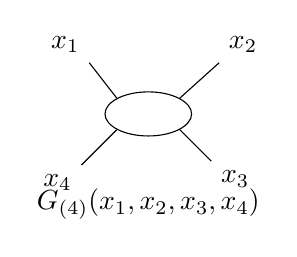
\begin{tikzpicture}[baseline=0]
\draw (0,0) ellipse (0.55 and 0.28);
\draw (-0.4,0.20)--(-0.75,0.65) node[above left] {$x_1$};
\draw (0.4,0.20)--(0.9,0.65) node[above right] {$x_2$};
\draw (0.4,-0.20)--(0.8,-0.6) node[below right] {$x_3$};
\draw (-0.4,-0.20)--(-0.85,-0.65) node[below left] {$x_4$};
\node at (0,-1.15) {$G_{(4)}(x_1,x_2,x_3,x_4)$};
\end{tikzpicture}
\end{adjustbox}
\qquad
$G_{(4)}\underset{\text{преобр. Фурье}}{\longrightarrow}
\underline{\text{ф-я от }p_1,p_2,p_3,p_4}$

в имп. прост.
\end{center}

($\sim$ рассеяние $4^{\text{х}}$ частиц)

Полюс $=$ [зачёркнуто:
\Unclear{GELFAND-P000806}{pole-cancellation}{неразборчивое выражение, возможно $m_0$}]
$m_c^2$

\underline{ф-я (3)} зависит лишь от $p_j^2$ и $p_i\cdot p_j$
(из Лоренц.-инвар.)

и сод. $\delta(p_1+p_2-p_3-p_4)$ (из сохр импульса)

Вершинная ф-я Грина:
\begin{equation*}
\Gamma=\frac{G(p_1,p_2,p_3,p_4)}{G(p_1)G(p_2)\ldots G(p_4)}.\tag{4}
\end{equation*}
(после вын. $\delta$-ф-и)

По теории возмущений (при $\lambda_0=0$) получим
\begin{equation*}
G^0(p)=\frac{1}{p^2+m^2}.\tag{5}
\end{equation*}

\SourcePage{GELFAND-P000807}{38}
% Обзор исходного PNG: 2440 x 3480; весь кадр и локальные области просмотрены непосредственно.
% Координаты ниже: (x0,y0,x1,y1), начало в левом верхнем углу исходного PNG;
% правая и нижняя границы не включены. scale — растровое увеличение ближайшим соседом,
% не повышение исходного разрешения. В журнале сохранены также расширенные и повторные окна.
% review upper: box=(180,0,2380,805); scale=1
% review middle: box=(130,790,2410,1640); scale=1
% review lower: box=(65,1630,2340,2760); scale=1
% review top-cancel: box=(265,80,415,180); scale=6
% review lambda-args: box=(360,325,1340,575); scale=3
% review denominator-cancel: box=(1000,960,1120,1120); scale=6
% review electrodyn-cancel: box=(995,1210,1125,1320); scale=6
% review beta-symbol: box=(400,1460,610,1640); scale=6
% review insertion: box=(70,2530,1875,2720); scale=3
[Зачёркнуто: \Unclear{GELFAND-P000807}{top-cancellation}{возможно $\Gamma(p)$}.]
\begin{equation*}
\frac{[G(p_1)\ldots G(p_4)]^{1/2}}{[G^0(p_1)\quad G^0(p_4)]^{1/2}}
\end{equation*}
\begin{equation*}
\lambda(p_i))=\lambda_0\Gamma(p_i))
\frac{[\prod_1^4G(p_i]^{1/2}}{[\prod_1^4G_0(p_i)]^{1/2}}
\quad\text{— \underline{заряд} (инвариантный)}
\end{equation*}
\Unclear{GELFAND-P000807}{lambda-arguments}{Аргументы $p$ / $p_i$; закрывающие скобки переписаны.}
[В числителе после $p_i$ видна квадратная скобка без отдельной круглой.]

$p=(p_1,p_2,p_3,p_4)$

$\lambda_0$ подб. так, чтобы физ. заряд был конечен (и все ф-и Грина тоже)

Парадокс \underline{Ландау и Померанчука}:
если не по теории возм., а оставить главный $\ln$, то получ.
\begin{equation*}
\lambda_\mu=\frac{\lambda_0}{1+\frac32\frac{\lambda_0}{16\pi^2}\ln\frac{\Lambda}{\mu^2}}.
\end{equation*}
[В знаменателе перед $\ln$ зачёркнуто:
\Unclear{GELFAND-P000807}{denominator-cancellation}{неразборчиво}.]

[Справа от формулы:]
$\mu$ — опр. точка: $p_ip_j=\mu^2$,
$p_i^2=(\ldots)\mu^2$.

$(\cdot)$ из $(\sum p_i)^2=0$.

\begin{equation*}
\lambda_0>0\quad\Rightarrow\quad\lambda_\mu\longrightarrow\infty
\quad\text{при }\Lambda\longrightarrow\infty
\quad\text{(т.е. снятии обрезания).}
\end{equation*}
\Unclear{GELFAND-P000807}{landau-limit}{Согласованность записанной формулы и предела.}

То же в кв. электродин.
[Зачёркнуто: \Unclear{GELFAND-P000807}{electrodynamics-cancellation}{неразборчиво}.]
(ни при какой затрав. $\lambda_0$ не получ. $\frac{1}{137}$)

Необходима асимптотика коэфф. в ряде теории возмущений,
возник. для
\begin{equation*}
\psi=\frac{d\lambda_\mu}{d\ln\frac{\Lambda}{\mu^2}}
=a_2\lambda_\mu^2+a_3\lambda_\mu^3+\ldots
\end{equation*}
асимпт. по $k$ при $k\to+\infty$ есть

Первые 4 члена найдены.

\underline{Идея:} метод Лапласа для континуального интеграла

\underline{Нер-во Соболева:}
\begin{equation*}
\left[\int(\partial_\sigma\varphi)^2\,d^4x\right]^2
\geq\frac{32\pi^2}{3}\int\varphi^4(x)\,d^4x
\end{equation*}
рав-во достигается при
\begin{equation*}
\varphi=\frac{c_1}{(x-x_0)^2+\lambda^2}
\end{equation*}

[\underline{Вставка Захарова}
\quad $\underline{\Delta\varphi+\varphi^3=0}$
— из ур-й Я.-М. получается]

\SourcePage{GELFAND-P000808}{unlabelled}
% Обзор исходного PNG: 2440 x 3480; весь кадр и локальные области просмотрены непосредственно.
% Координаты ниже: (x0,y0,x1,y1), начало в левом верхнем углу исходного PNG;
% правая и нижняя границы не включены. scale — растровое увеличение ближайшим соседом,
% не повышение исходного разрешения. В журнале сохранены также расширенные и повторные окна.
% review upper-text: box=(170,1090,2395,1830); scale=1
% review middle-text: box=(140,1800,2380,2635); scale=1
% review lower-text: box=(210,2590,2395,3470); scale=1
% review module-count: box=(660,1515,720,1598); scale=8
% review equiv-diagram: box=(550,1980,1205,2240); scale=3
% review section-region: box=(1430,2410,2110,2680); scale=3
% review projection-symbol: box=(420,2630,515,2740); scale=6
\underline{4.12.78г.}\qquad \underline{Сем. Гельфанда.}

\underline{\underline{A. Guichardet}}

\underline{\underline{Расширения предст. топ. групп.}}

1. \underline{Расш. модулей над дискр. группами.}

$E,F$ — 2 $G$ модуля

Расш. $E$ с помощью $F$ — это 3-й $G$-модуль $H$, такой что $H\supset F$ и
$H/F\cong E$ или точная послед.
\begin{equation*}
0\longrightarrow F\longrightarrow H\longrightarrow E\longrightarrow0.\tag{1}
\end{equation*}
2 расш. эквив., если $\exists$ изом., такой, что диагр. коммут.

\SourceFigure{GELFAND-P000808}{equivalence-diagram}{Коммутативная диаграмма из двух строк: сверху $0\to F\to H\to E\to0$, снизу $0\to F\to H'\to E\to0$. Между двумя $F$ и двумя $E$ стоят вертикальные знаки равенства; от верхнего $H$ к нижнему $H'$ идёт стрелка вниз. Сразу справа от верхнего $H$ зачёркнут знак, возможно ещё одна буква $H$.}

Тривиальное расширение:
\begin{equation*}
\underline{H=F\oplus E}
\end{equation*}
\underline{Сильное расширение:} (1) — сильное, если $\exists$ сечение
[зачёркнуто: $E\overset{s}{\longrightarrow}H$]

\begin{center}
\begin{adjustbox}{max width=\linewidth}
\begin{tikzcd}
H \arrow[r,"v"] & E \arrow[r] \arrow[l,bend left=35,"s"'] & 0
\end{tikzcd}
\end{adjustbox}
\end{center}

$\underline{v\cdot s=\mathrm{id}}$;
\underline{$s$ — морфизм групп} (а не \underline{$G$-модулей})

[Под словом «групп» вставлено: (абелевых).]

(если $s$ — морф. $G$-мод., то расширение тривиально)

Мн-во классов эквив. [вставлено над строкой: сильных] расширений:
$\underline{\operatorname{Ext}^1(E,F)}$

Метод: когомологии

$\operatorname{Hom}(E,F)$ — морф. групп

это $G$-модуль: действие задаётся так
\begin{equation*}
gu=g\circ u\circ g^{-1}
\end{equation*}

\SourcePage{GELFAND-P000809}{43}
% Обзор исходного PNG: 2440 x 3480; весь кадр и локальные области просмотрены непосредственно.
% Координаты ниже: (x0,y0,x1,y1), начало в левом верхнем углу исходного PNG;
% правая и нижняя границы не включены. scale — растровое увеличение ближайшим соседом,
% не повышение исходного разрешения. В журнале сохранены также расширенные и повторные окна.
% review upper: box=(150,0,2390,1070); scale=1
% review middle: box=(130,1030,2390,2240); scale=1
% review bottom: box=(100,2190,2390,3480); scale=1
% review first-heading: box=(325,45,460,150); scale=6
% review correspondence: box=(335,1110,1315,1235); scale=3
% review action-matrix: box=(630,1815,1260,2070); scale=4
% review representations-word: box=(900,2055,998,2165); scale=6
\underline{\underline{Опр.}}

$H^1(G,\operatorname{Hom}(E,F))$

\underline{1-коциклы}
\begin{equation*}
f:G\longrightarrow\operatorname{Hom}(E,F)
\end{equation*}
\begin{equation*}
f(gg')=f(g)+g\circ f(g')\circ g^{-1}.\tag{2}
\end{equation*}
$Z^1$ — все коциклы

1-кограницы ($B^1$).
\begin{equation*}
\exists\ u\in\operatorname{Hom}(E,F):\quad
f(g)=g\circ u\circ g^{-1}-u
\end{equation*}
\begin{equation*}
H^1\underset{\mathrm{def}}{=}Z^1/B^1.
\end{equation*}
Сущ. соответствие (вз. однозн.)
\begin{equation*}
H^1\cong\operatorname{Ext}^1(E,F)
\end{equation*}
По коциклу $\varphi$ постр. расширение:
\begin{equation*}
H=F\oplus E
\end{equation*}
\begin{equation*}
g(f,e)=(gf+\varphi(g)g\cdot e,\quad g\cdot e).\tag{3}
\end{equation*}
или в матрицах:
\begin{equation*}
\begin{pmatrix}
V_g&\varphi(g)U_g\\
0&U_g
\end{pmatrix}
\quad\text{— \underline{так строится действие}.}
\end{equation*}
$V_g,U_g$ — \Unclear{GELFAND-P000809}{representation-count}{2 / зачёркнутый знак}
предст. $G$ в соотв. пр-вах.

Отсюда можно получить опр. коцикла.

2 предст. эквив. $\Longleftrightarrow$ коциклы гомологичны

2. \underline{Расширения модулей над алгебрами Ли.}

[Справа:]
\begin{equation*}
X\longrightarrow\begin{pmatrix}A(X)&f(X)\\0&B(X)\end{pmatrix}
\end{equation*}
коцикл — линейное отображение
$f:\mathfrak g\longrightarrow\operatorname{Hom}(E,F)$

\underline{опр. коцикла} имеет вид:
\begin{equation*}
f([X,Y])=X\circ f(Y)-f(Y)\circ X-Y\circ f(X)+f(X)\circ Y.\tag{4}
\end{equation*}
$f$ — кограница, если $\exists\ u$
\begin{equation*}
f(X)=X\circ u-u\circ X.\tag{5}
\end{equation*}
\underline{Лемма 1.} $E,F$ имеют [вставлено над строкой: различные]
инфинитезим. характеры $\Rightarrow$
\begin{equation*}
\Rightarrow\quad\operatorname{Ext}^1(E,F)=0
\end{equation*}
$\mathfrak g\longmapsto U(\mathfrak g)$\qquad
универс. обёрт. алгебра, $Z(\mathfrak g)$ — её центр

\SourcePage{GELFAND-P000810}{unlabelled}
% Обзор исходного PNG: 2440 x 3480; весь кадр и локальные области просмотрены непосредственно.
% Координаты ниже: (x0,y0,x1,y1), начало в левом верхнем углу исходного PNG;
% правая и нижняя границы не включены. scale — растровое увеличение ближайшим соседом,
% не повышение исходного разрешения. В журнале сохранены также расширенные и повторные окна.
% review upper: box=(0,0,2410,1125); scale=1
% review middle: box=(20,1080,2410,2200); scale=1
% review bottom: box=(0,2155,2410,3480); scale=1
% review margin-mark: box=(1910,465,2025,580); scale=6
% review relation-sign: box=(885,970,960,1052); scale=8
% review ideas-evaluation: box=(235,2490,1490,2615); scale=3
% review final-parenthesis: box=(290,3225,2390,3370); scale=3
% review bottom-cancellation: box=(1340,3250,1475,3340); scale=6
% review lie-k: box=(220,2000,353,2080); scale=6
Пусть $\underline{u\in Z(\mathfrak g)}$ действует в $E$ как умн. на скаляр
\begin{equation*}
\underline{u\cdot e=\chi(u)e}
\end{equation*}
Тогда $\chi\in\operatorname{Hom}(Z(\mathfrak g),\mathbb C)$

\underline{это инфинит. характер.}

$H^1(\mathfrak g,\operatorname{Hom}(E,F))$ — \underline{есть}

$H^1(\mathfrak g,\mathfrak h,\operatorname{Hom}(E,F))$,\qquad
$\mathfrak h\subset\mathfrak g$

[Справа на поле:
\Unclear{GELFAND-P000810}{right-margin-mark}{изолированный неразборчивый знак}.]

(описывает расширения, тривиальные с точки зрения $\mathfrak h$).
\begin{equation*}
Z^1(\mathfrak g,\mathfrak h,\operatorname{Hom}(E,F))
=\{f\in Z^1(\mathfrak g,\ldots),\quad f|_{\mathfrak h}=0\}
\end{equation*}
\begin{equation*}
H^1(\mathfrak g,\mathfrak h,\ldots)\in H^1(\mathfrak g,\ldots).
\end{equation*}
\Unclear{GELFAND-P000810}{relative-relation}{В источнике между группами написан знак $\in$.}

\underline{Комментарии:}

\underline{Можно с пом. дифференциала:}
\begin{equation*}
(df)(x,y)=f([x,y])-xf(y)+yf(x)
\end{equation*}
$xf(y)$ — \underline{\underline{действие}} алг. Ли

(выше запис. с пом. \underline{коммутатора})

3. \underline{Расширения модулей над группами Ли.}

$G$-модуль — топ. вект. пр-во, $G$ действ. непрерывно.

$\mathfrak g$ — алг. Ли

$K\subset G$

макс. комп. подгр.,

$\mathfrak k$ — соотв. алг.

$E,F$ — т.в.п.

\underline{1-я идея.}\quad \underline{коциклы}
\begin{equation*}
f:G\longrightarrow\operatorname{Hom}(E,F)
\end{equation*}
$(e,g)\longmapsto f(g)e$\qquad непр. по $g$ и $e$.

\underline{2-я идея:} вместо $E,F$ — пр-во дифф. векторов $E_\infty,F_\infty$

хороши, но не совершенны при $\underline{\underline{E=\mathbb C}}$.
Пусть так.

\underline{Теорема:}
\begin{equation*}
H^1(G,F)\underset{\substack{\swarrow\\\text{Delorme — Blanc}}}{\cong}
H^1(G,F_\infty)\underset{\substack{\downarrow\\\text{Van Est}}}{\cong}
H^1(\mathfrak g,\mathfrak k,F_\infty)
\end{equation*}

\underline{Для $\mathbb R$ нетрив.}
\begin{equation*}
\begin{pmatrix}1&at\\0&1\end{pmatrix}
\quad\text{— \underline{расширение} трив. $\mathbb R$-модуля тривиальным}
\end{equation*}
нет соотв. предст. групп и алгебр

(\underline{в когом.}: надо брать когом., трив.
[зачёркнуто: \Unclear{GELFAND-P000810}{bottom-cancellation}{неразборчиво}]
на компактной подгруппе).

\SourcePage{GELFAND-P000811}{44}
% Обзор исходного PNG: 2440 x 3480; весь кадр и локальные области просмотрены непосредственно.
% Координаты ниже: (x0,y0,x1,y1), начало в левом верхнем углу исходного PNG;
% правая и нижняя границы не включены. scale — растровое увеличение ближайшим соседом,
% не повышение исходного разрешения. В журнале сохранены также расширенные и повторные окна.
% review upper: box=(150,0,2420,1115); scale=1
% review middle: box=(210,1100,2420,2180); scale=1
% review lower: box=(170,2160,2420,2860); scale=1
% review bottom: box=(190,2830,2420,3475); scale=1
% review heading: box=(205,30,635,130); scale=3
% review dimension-sign: box=(2135,135,2225,220); scale=8
% review affine-mark: box=(1280,245,1370,330); scale=6
% review semisimple-cancel: box=(1390,570,1545,660); scale=6
% review nonsemisimple: box=(330,935,1050,1040); scale=3
% review counterexample-cancel: box=(895,1440,1020,1535); scale=6
% review second-margin-cancel: box=(260,1640,350,1715); scale=6
% review long-cancellations: box=(270,1900,1100,2145); scale=3
% review k-cancellations: box=(1160,2180,2260,2360); scale=3
% review product-notation: box=(1005,2910,1165,3030); scale=6
% review equality-mark: box=(940,2930,1008,3035); scale=8
% review nonunitary: box=(360,1135,1670,1225); scale=3
% review lower-cancel-detail: box=(425,2020,1080,2140); scale=4
% review k-cancel-left: box=(1180,2290,1560,2355); scale=6
% review k-cancel-right: box=(1610,2290,2145,2355); scale=6
% review relative-subalgebra: box=(635,2580,809,2745); scale=6
\underline{Несовершенство:}

даже если $F$ — неприв. унит. предст., то может быть
$\underline{\dim H^1(G,F)\ \text{\Unclear{GELFAND-P000811}{dimension-sign}{= / ≤}}\ +\infty}$

\underline{Пример}\qquad $G$ — афф. гр. прямой\qquad
\Unclear{GELFAND-P000811}{affine-mark}{R / зачёркнутый знак}\quad $ax+b$

$B^1$ всюду плотно в $Z^1$, но $\underline{\dim Z^1/B^1=+\infty}$

Причина: $F$ слабо содержит тривиальное предст.

Для полупростых групп всё хорошо.
[Зачёркнуто: \Unclear{GELFAND-P000811}{semisimple-cancellation}{неразборчиво}.]

Пусть $G$ — полупростая;

\underline{унит. неприв. предст.}

Известно, когда $H^1=0$.

Для неполупростых:
\begin{equation*}
\underline{SO_0(m,n)}
\end{equation*}
не сущ. неунит. предст. с ненулевыми когом.

\Unclear{GELFAND-P000811}{nonsemisimple-context}{Рубрика «Для неполупростых» и сокращение «неунит.» сохранены.}

\underline{Доб. недостаток $1^{\text{й}}$ идеи.}

Лемма об инфинит. хар. неверна!

Контрпример есть [зачёркнуто:
\Unclear{GELFAND-P000811}{counterexample-cancellation}{возможно «все»}]
для $SL(2,\mathbb R)$

\underline{2-я идея:} верна лемма об инфин. хар-рах, но

[На левом поле зачёркнуто:
\Unclear{GELFAND-P000811}{second-margin-cancellation}{возможно «но»}.]
\begin{equation*}
H^1(G,\operatorname{Hom}(E_\infty,F_\infty))
\end{equation*}
трудно вычислить.

\begin{equation*}
L_\infty^2\longrightarrow L_\infty^2
\end{equation*}
[Слева от этой формулы и строкой ниже — зачёркнутые записи; в нижней различимо «Задача».]
\Incomplete{GELFAND-P000811}{long-cancellations}{Зачёркнутые записи не прочитаны полностью; в верхней возможно $L_\infty^2$, после «Задача» дальнейший текст и знаки не установлены.}

\underline{3-я идея.}
\begin{equation*}
E,F\rightsquigarrow E_K,F_K
\end{equation*}
(векторы, включ. в конечномерные предст. $K$).

\Incomplete{GELFAND-P000811}{k-cancellations}{Под скобкой о векторах находятся два густо перечёркнутых текстовых фрагмента; исходные слова не читаются.}

$K$-конечные;\qquad \underline{$K$ — макс. комп. подгруппа}

$SL(2,\mathbb R)$ — для всех непр. модулей Хариш-Чандры можно выч.
\begin{equation*}
H^1(\mathfrak g,\mathfrak k,\operatorname{Hom}(E_K,F_K))
\end{equation*}
алгебра без топологии.

4. \underline{Случай полупрямого произведения.}
\begin{equation*}
G=B\underset{\text{полупр.}}{\times}A
\underset{\text{\Unclear{GELFAND-P000811}{product-equality-mark}{σ / g}}}{=}
B\wedge A;\qquad B=\mathbb R^n,\quad A\text{ — гр. Ли}
\end{equation*}
(напр., афф. гр. прямой).

$B^*$ — сопр. пр-во,\qquad $\langle b,x\rangle$ — двойств.

$X=A$-орбита в $B^*$

(действие $A$ в $B$ есть и опр. полупрямого произвед.)

\SourcePage{GELFAND-P000812}{unlabelled}
% Обзор исходного PNG: 2440 x 3480; весь кадр и локальные области просмотрены непосредственно.
% Координаты ниже: (x0,y0,x1,y1), начало в левом верхнем углу исходного PNG;
% правая и нижняя границы не включены. scale — растровое увеличение ближайшим соседом,
% не повышение исходного разрешения. В журнале сохранены также расширенные и повторные окна.
% review upper: box=(160,0,2390,890); scale=1
% review second: box=(210,860,2390,1720); scale=1
% review third: box=(190,1660,2390,2490); scale=1
% review bottom: box=(230,2450,2390,3475); scale=1
% review date-cancel: box=(260,45,360,135); scale=6
% review list-cancel: box=(255,678,374,810); scale=6
% review feynman-title: box=(727,775,1680,864); scale=3
% review prize-word: box=(1415,1710,1750,1805); scale=3
% review group-letter: box=(450,2330,820,2630); scale=4
% review final-argument: box=(525,3180,590,3250); scale=8
% review final-argument-corrected: box=(510,3240,590,3315); scale=8
% review feynman-hibbs: box=(1055,427,1322,520); scale=3
% review prize-full: box=(1035,1710,1780,1805); scale=3
[Слева от даты зачёркнуто: \Unclear{GELFAND-P000812}{date-cancellation}{неразборчиво}.]

\underline{\underline{12/II-79 г.}}\qquad \underline{Сем. Гельфанда.}

\underline{Что нужно знать?} (по \underline{А. А. Белавину}):

I. \underline{Фейнман}.

1. Курс для домохозяек, гл. 8, 9.

2. Статистическая физика

3. Интегралы по путям (с Гиббсом)

II. \underline{Хуанг} «Статист. механика» Глава: Решение Онзагера.

III. \underline{Ф. Клейн} «Лекции по истории математики в \underline{XIX} столетии»

[Зачёркнут номер: \Unclear{GELFAND-P000812}{list-cancellation}{возможно IV}. Следующая вставка охвачена слева скобкой; из-под зачёркнутого номера идёт стрелка по левому полю к промежутку перед II.]

[4. Книжки с синими кубиками на обложке (на белом фоне)

(Фейнман: «Фунд. зак. физики»).]

IV. \underline{Дирак} Статья в книге «Монополь Дирака»

книги. «Лекции по квантовой механике»

«[Знаки повтора слов «Лекции по»] теории поля»

«Общая теория относительности»

V. \underline{Ахиезер}, \underline{Берестецкий} «Квантовая электродинамика»

(надо знать содержание, но не читать)

VI. Сборник «Частицы и компенсирующие поля», Статья \underline{Янга и Миллса}.

VII. \underline{Коноплёва}, \underline{Попов}: «Калибровочные поля» (часть, написанная Поповым)

\underline{Белавин}

Задача, выдв. на конкурс черноголовским королевским физ. об-вом: или

Что осталось нереш. об инстантонах?

$A,B$ — 2 кватернионные матрицы $N\times(N+1)$

Надо найти такую параметризацию [вставлено над строкой: «таких»] пар матриц $A$ и $B$, что
если $M=xA+B$, то $MM^+$ вещественна (при любом кватернионе $x$),
с точностью до действия группы
\begin{equation*}
GMV
\end{equation*}
\Unclear{GELFAND-P000812}{group-letter}{Буква после $GM$ и в двух следующих записях: $V$ / $U$ / $\upsilon$.}
\begin{equation*}
\begin{aligned}
G&\qquad N\times N\\
V&\qquad (N+1)\times(N+1)\qquad VV^+=1
\end{aligned}
\end{equation*}
Всего должно быть $8N-3$ параметров.

Надо найти красивую параметризацию таких матриц.

\underline{О некоторых точно решаемых 2-мерных задачах КТП.}

Наивный аргумент по поводу \underline{невылетания}. (Вильсон)
\begin{equation*}
\psi(x)\qquad S[\psi,\ldots]\text{ — действие},\qquad \delta S=0\text{ — ур-я движ.}
\end{equation*}
\begin{equation*}
\psi(x)\longrightarrow e^{i\alpha(x)}\psi(x)\qquad\text{— калибр. инвариантность}
\end{equation*}
\Unclear{GELFAND-P000812}{final-argument}{В левой части последней формулы аргумент $x$ наведён по более ранним штрихам; первоначальный знак не установлен.}

\SourcePage{GELFAND-P000813}{63}
% Обзор исходного PNG: 2440 x 3480; весь кадр и локальные области просмотрены непосредственно.
% Координаты ниже: (x0,y0,x1,y1), начало в левом верхнем углу исходного PNG;
% правая и нижняя границы не включены. scale — растровое увеличение ближайшим соседом,
% не повышение исходного разрешения. В журнале сохранены также расширенные и повторные окна.
% review upper: box=(185,15,2370,920); scale=1
% review second: box=(170,915,2370,1720); scale=1
% review third: box=(65,1700,2380,2530); scale=1
% review bottom: box=(65,2510,2380,3450); scale=1
% review correlation-cancel: box=(1452,225,1537,300); scale=6
% review hidden-heading: box=(260,325,1055,422); scale=3
% review integral-word: box=(890,423,1362,535); scale=3
% review spectrum: box=(660,690,1150,795); scale=3
% review sigma-site: box=(895,1060,1010,1223); scale=6
% review bottom-cancel: box=(329,3158,544,3250); scale=4
% review hamiltonian-sums: box=(430,799,1220,990); scale=3
% review commutator-coefficient: box=(1260,2220,1830,2410); scale=3
% review correlation-cancel-full: box=(1390,215,1498,300); scale=6
% review integral-word-again: box=(940,433,1370,525); scale=6
% review chain-dots: box=(900,1015,1430,1120); scale=3
% review commutator-coefficient-corrected: box=(665,2240,1020,2420); scale=4
% review fermion-normalization: box=(360,2605,940,2770); scale=3
% review fermion-delta: box=(825,3000,1040,3130); scale=5
% review correlation-word: box=(405,210,820,315); scale=3
\begin{equation*}
\langle\psi(x)\overline{\psi(y)}\rangle
=e^{i(\alpha(x)-\alpha(y))}\langle\ldots\rangle
\end{equation*}
$\Rightarrow$ корреляц. ф-и 0 $\Rightarrow$ невозможность
[зачёркнуто: \Unclear{GELFAND-P000813}{correlation-cancellation}{неразборчиво}]
для заряж. объектов.

\underline{Доклад о скрытой симметрии.}

Переход от конт. инт. к многократному может нарушить симметрию.

1) Имеется теория
\begin{equation*}
\Box\varphi=\sin\varphi,\qquad \varphi(x,t),\qquad
\Box=\frac{\partial^2}{\partial t^2}-\frac{\partial^2}{\partial x^2}
\end{equation*}
получен квазикласс. спектр.

2) Далее, есть гам. (\underline{Baxter})!
\begin{equation*}
H=\sum_{n=1}^N\sum_{\alpha=1}^3 J_\alpha\sigma_n^\alpha\sigma_{n+1}^\alpha \tag{1}
\end{equation*}
[Над следующей формулой:]
\begin{center}
\begin{adjustbox}{max width=\linewidth}
\begin{tikzpicture}
\draw (0,0) circle (0.045);
\fill (0.55,0) circle (0.035);
\fill (1.15,0) circle (0.035);
\fill (1.70,0) circle (0.035);
\fill (2.20,0) circle (0.035);
\fill (2.75,0) circle (0.035);
\fill (3.80,0) circle (0.035);
\node at (0,-0.3) {$1$};
\node at (0.55,-0.3) {$2$};
\node at (1.15,-0.3) {$3$};
\node at (1.70,-0.3) {$.$};
\node at (2.20,-0.3) {$.$};
\node at (3.80,-0.3) {$N$};
\end{tikzpicture}
\end{adjustbox}
\end{center}
\begin{equation*}
\sigma_n^\alpha=1\otimes1\otimes\ldots\otimes
\underset{\text{\Unclear{GELFAND-P000813}{sigma-site}{n / зачёркнутый знак}}}{\sigma^\alpha}
\otimes1\otimes\ldots\otimes1.\qquad \alpha=1,2,3
\end{equation*}
[Справа:] (1-мерная кв. цепочка)

\fbox{$N+1=1$} — условие периодичности.
\begin{equation*}
\sigma^3=\begin{pmatrix}1&0\\0&-1\end{pmatrix},\quad
\sigma^1=\begin{pmatrix}0&1\\1&0\end{pmatrix},\quad
\sigma^2=\begin{pmatrix}0&-i\\i&0\end{pmatrix};\qquad J_\alpha\in\mathbb R
\end{equation*}
$H$ — матрица $2^N\times2^N$

\underline{Задача}: найти соб. вект. и соб. значения.

По смыслу: эти модели аналогичны 4-мерн. калибр. теориям.

При пред. переходе из 2) получ. $\sin$-Гордон.

Сист. (1) решил Бакстер

Сам Гамильтониан — Гейзенберга. (анизотропный — из-за $J_\alpha$ — ферромагнетик Гейзенберга)

(или $XYZ$-модель)

Лютер свел (1) к модели Тирринга.

Вып. соотношения:
\begin{equation*}
\begin{cases}
[\sigma_n^\alpha,\sigma_m^\beta]=0,\qquad n\ne m\\
[\sigma_n^\alpha,\sigma_n^\beta]=\varepsilon_{\alpha\beta\gamma}\,\sigma_n^\gamma\\
[\sigma_n^1,\sigma_n^2]_+=0
\end{cases}\tag{2}
\end{equation*}
$[\ ,\ ]_+$ — антикоммутатор

\Unclear{GELFAND-P000813}{commutator-normalization}{В средней строке (2) перед $\varepsilon_{\alpha\beta\gamma}$ коэффициента не написано.}

Сделаем решёточные фермионы.
\begin{equation*}
\psi_n^\pm=(\sigma_n^1\pm i\sigma_n^2)\prod_{m=1}^{n-1}\sigma_m^3;\tag{3}
\end{equation*}
это фермионы, т. е.
\begin{equation*}
\begin{cases}
[\psi_n^+,\psi_m^+]_+=0\\
[\psi_n^-,\psi_m^+]_+=\delta_{nm}
\end{cases}\tag{4}
\end{equation*}
\Unclear{GELFAND-P000813}{fermion-normalization}{В (3) нет числового множителя перед скобкой; в (4) справа стоит $\delta_{nm}$.}

В [зачёркнуто: \Unclear{GELFAND-P000813}{bottom-cancellation}{неразборчивое слово}]
действит. — так Онзагер решил модель Изинга:

выразим $\sigma$ через $\psi$: $H$ станет квадр. и всё диагонализуется

\SourcePage{GELFAND-P000814}{unlabelled}
% Обзор исходного PNG: 2440 x 3480; весь кадр и локальные области просмотрены непосредственно.
% Координаты ниже: (x0,y0,x1,y1), начало в левом верхнем углу исходного PNG;
% правая и нижняя границы не включены. scale — растровое увеличение ближайшим соседом,
% не повышение исходного разрешения. В журнале сохранены также расширенные и повторные окна.
% review upper: box=(80,15,2410,925); scale=1
% review second: box=(100,905,2335,1700); scale=1
% review third: box=(80,1680,2340,2440); scale=1
% review bottom: box=(75,2400,2360,3435); scale=1
% review assertion-cancel: box=(245,265,594,345); scale=4
% review equivalence-abbreviation: box=(470,733,855,815); scale=3
% review sigma-cancel: box=(293,1410,535,1524); scale=4
% review quartic-term: box=(915,1780,1440,1910); scale=4
% review boson-exponent: box=(337,2560,1100,2750); scale=3
% review names: box=(297,3060,1540,3200); scale=3
% review symbol-index: box=(686,3165,970,3265); scale=5
% review quartic-index: box=(1161,1856,1210,1907); scale=8
% review canonical-rhs: box=(775,2460,1045,2570); scale=5
% review boson-field: box=(655,2590,720,2675); scale=8
Сделаем пр. Фурье
\begin{equation*}
\widetilde\psi_k^\pm=\sum_n\psi_n^\pm e^{ikn}\tag{5}
\end{equation*}
[Зачёркнуто: \Unclear{GELFAND-P000814}{assertion-cancellation}{сформулирую / сформулируем}.]
\underline{Утверждение}.
\begin{equation*}
H=\sum_n(\sigma_n^1\sigma_{n+1}^1+\Delta\sigma_n^3),\qquad
\Delta\text{ — число}\tag{6}
\end{equation*}
\begin{equation*}
\dot\sigma_n(t)=i[\sigma_n,H]\tag{7}
\end{equation*}
— ур-я движения; для решений $\forall t$ вып. коммут. соотн. (2)
\begin{equation*}
\sigma_n(0)=\sigma_n.
\end{equation*}
После замены ур-я стан. линейными (по $\psi$)

$\Rightarrow$ это эквив. нах. соб. векторов.

($\sigma$ можно выразить через $\psi$)

Получ. ур-я
\begin{equation*}
\dot\psi_n=\psi_{n+1}-\psi_{n-1}\tag{8}
\end{equation*}
Выраж. гамильтониана \underline{в исх. задаче}.
\begin{equation*}
H\sim\sum_n\bigl(\psi_n\psi_{n+1}^+-\psi_n^+\psi_{n+1}
+\psi_n^+\psi_n\psi_{n+1}^+\psi_{n+1}\bigr)\tag{9}
\end{equation*}
[Зачёркнуто: \Unclear{GELFAND-P000814}{sigma-cancellation}{$\sigma_1$ и $\sigma_2$ / $\sigma^1$ и $\sigma^2$}.]
$\sigma_n$ выраж. через $\psi$ по индукции.

(9) — гамильт. реш. модели Тирринга (уже нелин.)

Переход к непрерывному случаю: получаем
\begin{equation*}
\int dx\left[\psi_1^+(x)\frac{\partial\psi_2(x)}{\partial x}
+\psi_1^+\psi_2\psi_1^+\psi_2^+
+\text{э. с.}\right]\tag{10}
\end{equation*}
[После четвёрного произведения зачёркнута закрывающая квадратная скобка «]»; «+ э. с.» вписано до новой скобки. Под «э. с.» подписано: «эрмитово сопр.».]

\Unclear{GELFAND-P000814}{quartic-term}{В четвёрном произведении третья $\psi$ имеет наведённый нижний индекс $1$; плюсы при первом, третьем и четвёртом множителях сохранены.}
\begin{equation*}
\underline{x=na},\qquad\psi(x)\approx\psi_n
\end{equation*}
$\psi_1,\psi_2$ — из различ. \underline{чётных} и \underline{нечётных} узлов решётки

\underline{1975}\qquad \underline{Мандельстам} и\ldots:
\underline{кв. модель Тирринга $\sim$ кв. мод. $\sin$-Гордон}

\underline{кв. мод. $\sin$-Горд}
\begin{equation*}
\Box\varphi=\sin\varphi\tag{11}
\end{equation*}
\begin{equation*}
[\dot\varphi(t,x),\varphi(t,y)]=\delta(x-y)\tag{12}
\end{equation*}
\begin{equation*}
\psi=i e^{i\alpha\Phi+\beta\int_{-\infty}^x\dot\Phi(y)\,dy}\tag{13}
\end{equation*}
\Unclear{GELFAND-P000814}{bosonization-notation}{В (13) знаки поля имеют вид $\Phi$ / $\varphi$; перед $e$ стоит $i$, а перед $\beta$ дополнительного $i$ не видно.}

$\Downarrow$\qquad (при $\alpha\beta=4\pi$)
\begin{equation*}
[\psi(x),\psi^+(y)]_+=\delta(x-y)\tag{14}
\end{equation*}
\Unclear{GELFAND-P000814}{canonical-normalization}{В правой части (12) записано $\delta(x-y)$ без множителя $i$.}

Конец введения.

\underline{Саша Замолодчиков}. Алгебра Замолодчикова.

[Под именем:] (Москва)
\begin{equation*}
A_i(\theta),\qquad 1\le i<M
\end{equation*}
[Под $A_i(\theta)$ с короткой чертой-указателем:] символы

\SourcePage{GELFAND-P000815}{64}
% Обзор исходного PNG: 2440 x 3480; весь кадр и локальные области просмотрены непосредственно.
% Координаты ниже: (x0,y0,x1,y1), начало в левом верхнем углу исходного PNG;
% правая и нижняя границы не включены. scale — растровое увеличение ближайшим соседом,
% не повышение исходного разрешения. В журнале сохранены также расширенные и повторные окна.
% review upper: box=(75,5,2350,805); scale=1
% review middle: box=(60,765,2320,1710); scale=1
% review lower: box=(70,1680,2340,2705); scale=1
% review bottom-margin: box=(0,2630,2440,3480); scale=1
% review exchange-indices-left: box=(422,115,1120,285); scale=4
% review exchange-indices-right: box=(1260,156,1835,305); scale=4
% review index-range: box=(299,275,920,365); scale=4
% review m-cancel: box=(303,392,364,475); scale=8
% review elliptic: box=(400,1265,932,1668); scale=3
% review transfer-indices: box=(284,1905,1690,2123); scale=3
% review commutator-cancel: box=(578,2220,657,2344); scale=6
% review margin-angle: box=(120,2610,270,2690); scale=5
% review margin-angle-full: box=(110,2595,300,2760); scale=4
% review top-edge-mark: box=(0,0,65,85); scale=6
[В самом верхнем левом углу — отдельный короткий вертикальный штрих с небольшим загибом вправо наверху.]

Можно писать произведения
\begin{equation*}
A_i(\theta_1)A_\alpha(\theta_2)
=S_{ik}^{\alpha\beta}(\theta_1-\theta_2)A_\beta(\theta_2)A_k(\theta_1)\tag{15}
\end{equation*}
\begin{equation*}
1\le\beta<M,\qquad 1\le\alpha<M.
\end{equation*}
[Зачёркнут небольшой знак: \Unclear{GELFAND-P000815}{m-cancellation}{неразборчиво}.]
\underline{$M=2$}
\begin{equation*}
\begin{cases}
A_1A_1=aA_1A_1+dA_2A_2\\
A_1A_2=bA_2A_1+cA_1A_2
\end{cases}\tag{16}
\end{equation*}
и ещё 2 соотн., получ. заменой 1 на 2.

\Unclear{GELFAND-P000815}{index-range}{В диапазонах индексов перед $M$ стоят строгие знаки $<$; ниже при $M=2$ используется $A_2$.}

Ещё надо совместить с ассоциативностью.

\underline{На $S$ наложено соотв. условие}
\begin{equation*}
\bigl(A_1(\theta_1)A_1(\theta_2)\bigr)A_2(\theta_3)
=A_1(\theta_1)\bigl(A_1(\theta_2)A_2(\theta_3)\bigr)
\end{equation*}
Ур-я прив. к факторизации многочастичных $S$-матриц

Так он нашёл $S$-матрицу $\sin$-Gordon и т. д.

\underline{Ур-я для} $a,b,c,d$ (из (16)) \underline{явно решаются} (!)
\begin{equation*}
\begin{cases}
a=\operatorname{sn}(\theta+\eta,k)\\
b=\operatorname{sn}(\theta-\eta,k)\\
c=\operatorname{sn}(2\eta,k)\\
d=k\cdot abc
\end{cases}\tag{17}
\end{equation*}
\Unclear{GELFAND-P000815}{elliptic-parameter}{Второй параметр $\operatorname{sn}$ и множитель в $d$: $k$ / $\kappa$.}

\underline{Это все реш. с точн. до множителя.}

Baxter исп. такие объекты
\begin{equation*}
T^{\alpha_1,\beta_1,\ldots,\alpha_N,\beta_N}(\theta)
=S_{i_1i_2}^{\alpha_1\beta_1}S_{i_2i_3}^{\alpha_2\beta_2}
\ldots S_{i_Ni_1}^{\alpha_N\beta_N}\tag{18}
\end{equation*}
Получилась $2^N\times2^N$-матрица. Оказ., что

[Слева от (19) зачёркнуто: \Unclear{GELFAND-P000815}{commutator-cancellation}{неразборчивый знак}.]
\begin{equation*}
[T(\theta),H]=0\tag{19}
\end{equation*}
($\Rightarrow$ беск. набор инт. дв-ния)
\begin{equation*}
[T(\theta_1),T(\theta_2)]=0\tag{20}
\end{equation*}
($\Rightarrow$ в инволюции)

На самом деле он точно решил.

\SourceFigure{GELFAND-P000815}{margin-angle}{Внизу слева от последней строки — фрагмент углообразной пометы: длинный штрих поднимается вправо, затем коротко идёт вниз; под ним видна вершина малого уголка. Нижние части обрываются на общей горизонтальной границе. Полная форма и назначение не установлены.}
\SourcePage{GELFAND-P000816}{unlabelled}
% Осмотрен оригинал 2440 x 3480. Координаты: (x0,y0,x1,y1),
% начало в левом верхнем углу, правая и нижняя границы исключены.
% Верхнее поле до y=1090 осмотрено; уверенно читаемого номера листа нет.
% heading (315,1090,1430,1550), 3x; eq1 (420,1540,1880,1685), 3x.
\underline{\underline{19/II-79г.}}\qquad \underline{Сем. Гельфанда.}

\underline{\underline{Белавин.}}

\begin{equation*}
A_i(\theta),\quad 1\leq i\leq M,\quad\text{--- символы}
\end{equation*}
$\theta$ --- параметр

% Заголовок в источнике подчёркнут волнистой линией.
\underline{Алгебра Замолодчикова.}

\begin{equation*}
(1)\qquad A_i(\theta_1)A_\alpha(\theta_2)
=S_{ik}^{\alpha\beta}(\theta_1-\theta_2)A_\beta(\theta_2)A_k(\theta_1)
\end{equation*}

% assoc (395,1685,2380,1920), 3x; verb (1380,1685,1720,1770), 8x.
% Conjunction но: (1105,2390,1300,2485), 8x.
Требуется и ассоциативность. Тогда возникают кубические соотн.

\begin{equation*}
A_i(\theta_1)A_j(\theta_2)A_k(\theta_3)
\end{equation*}
[Справа:] (своб. ассоц. алгебра, порожд.
$M$ \Unclear{GELFAND-P000816}{free-algebra-word}{коммутирующими перем.} с соотн.)

% interp (375,1905,1920,2555), 2x; simple-diagram (390,2010,860,2130), 5x.
Интерпретация (физическая)

\begin{center}
\begin{adjustbox}{max width=\linewidth}
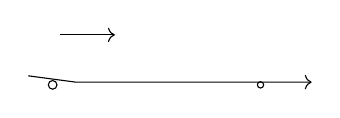
\begin{tikzpicture}[x=1cm,y=1cm]
\draw[->] (0.4,0.6) -- (1.1,0.6);
\draw[->] (0,0.08) -- (0.6,0) -- (3.6,0);
\draw (0.31,-0.035) circle (0.055);
\draw (2.95,-0.035) circle (0.04);
\end{tikzpicture}
\end{adjustbox}
\end{center}

\Unclear{GELFAND-P000816}{particle-word}{полос. / полюс.} --- частицы,
$\theta_i$ --- скорости

$A_iA_\alpha$ --- $i$-я част. левее

$\theta_1>\theta_2\ \Rightarrow$ догонит $i$-я.

Могут догонять по разному, но важны начало и конец
(что в промежутке --- не важно)

% collisions (270,2520,1375,2870), 3x.
\SourceFigure{GELFAND-P000816}{collision-diagrams}{Два рисунка со знаком равенства между ними. На каждом ось $x$ направлена вверх, ось $t$ вправо и изображены три попарно пересекающиеся линии. Слева подписи $\theta_2$ у пологой восходящей линии, $\theta_1$ под крутой восходящей линией, $\theta_3$ справа от нисходящей линии. Справа подписи $\theta_2$ и $\theta_1$ внизу, $\theta_3$ у верхнего левого конца нисходящей линии. Видны стрелки вверх и вправо на восходящих линиях и вверх и влево на линии $\theta_3$. Требуют проверки поправленные штрихи и наконечники стрелок, особенно на левой линии $\theta_3$.}

% chain1 (355,2890,2020,3050), 3x; chain2 (375,3060,1960,3240), 3x;
% chain3 (360,3230,2010,3425), 3x.
\begin{align*}
\bigl(A_i(\theta_1)A_j(\theta_2)\bigr)A_k(\theta_3)
&=S_{ii_1}^{jj_1}A_{j_1}(\theta_2)
  \bigl(A_{i_1}(\theta_1)A_k(\theta_3)\bigr)=\\
&=S_{ii_1}^{jj_1}(\theta_{12})S_{i_1i_2}^{kk_1}(\theta_{13})
  \bigl(A_{j_1}(\theta_2)A_{k_1}(\theta_3)\bigr)A_{i_2}(\theta_1)=\\
&=S_{ii_1}^{jj_1}(\theta_{12})S_{i_1i_2}^{kk_1}(\theta_{13})
  S_{j_1j_2}^{k_1k_2}(\theta_{23})A_{k_2}(\theta_3)A_{j_2}(\theta_2)A_i(\theta)
\end{align*}
\Unclear{GELFAND-P000816}{chain-first-aj}{[Буква $A$ во втором множителе $A_j(\theta_2)$ в начале цепочки обведена; прежнее начертание не устанавливается.]}

\Unclear{GELFAND-P000816}{chain-first-s}{[В первой строке после $S_{ii_1}^{jj_1}$ аргумент не виден.]}

% Third S upper indices: (1000,3220,1225,3340), 8x, separate 1 is visible after first k.

\Unclear{GELFAND-P000816}{chain-reworked-theta}{[В последней строке у $A_{k_2}$ знак $\theta$ в аргументе $\theta_3$ обведён; прежнее начертание не устанавливается.]}

\Unclear{GELFAND-P000816}{chain-last-factor}{[Последний множитель читается $A_i(\theta)$; дополнительных цифровых индексов не видно.]}

\SourcePage{GELFAND-P000817}{67}
% Direct inspection of original 2440 x 3480 PNG. Crop coordinates in ledger
% are original pixels, [left, top, right, bottom), with enlargement factors.
\underline{Ур-я приобр. вид:}
\begin{equation*}
\begin{aligned}
(2)\quad &S^{kk_1}_{ii_1}(\theta)S^{jj_1}_{i_1i_2}(\theta+\theta')
S^{j_1j_2}_{k_1k_2}(\theta')\\
&{}=S^{jj_1}_{kk_1}(\theta')S^{j_1j_2}_{ii_1}(\theta+\theta')
S^{k_1k_2}_{i_1i_2}
\end{aligned}
\end{equation*}
\Unclear{GELFAND-P000817}{eq2-index-arguments}{Индексы и отсутствие аргумента у последнего $S$ в (2) сохранены буквально.}
По $i_1,j_1,k_1$ суммир.

Итого: $M^6$ ур-й на $M^4$ ф-й $S^{\alpha\beta}_{ik}(\theta)$

$S$ играет роль $S$-матрицы.

Положим
\begin{equation*}
(3)\quad
T_{\vec{\alpha},\vec{\beta}}(\theta)=
S^{\alpha_1\beta_1}_{i_1i_2}(\theta)
S^{\alpha_2\beta_2}_{\text{\Unclear{GELFAND-P000817}{eq3-middle-subscript}{$i_2i_3$}}}(\theta)
% В (3) четыре отдельные точечно-штриховые отметки: [955,790,1110,845), 4×, исходные пиксели.
\cdot\;\cdot\;\cdot\;\cdot
S^{\alpha_N\beta_N}_{\text{\Unclear{GELFAND-P000817}{eq3-final-subscript}{$i_Ni_1$ / $i_Nk_1$}}}(\theta)
\end{equation*}
Получится матрица $M^N\times M^N$
(„трансфер-матрица“)

% Справа от определения матрицы.
$(\alpha_1,\ldots,\alpha_N)$ — индексы.

$(\beta_1,\ldots,\beta_N)$ — 2-й набор инд.

Утверждается, что
\begin{equation*}
(4)\quad [T(\theta),T(\theta')]=0
\end{equation*}
% На строке (4) справа от нуля.
\Unclear{GELFAND-P000817}{eq4-crossed-right}{густо зачёркнутая запись неразборчива}

(в силу ур-й факторизации).

% Слева между (4) и следующей строкой.
\Unclear{GELFAND-P000817}{eq4-crossed-left}{зачёркнутая подчёркнутая запись неразборчива}

Факториз. $S$-матр. — следствие кон. числа законов сохр.

\underline{Явная запись ур-й при $M=2$}

(случай ур-й Максвелла)
\begin{equation*}
(5)\quad
\left\{
\begin{aligned}
A_1A_1&=a\,A_1A_1+d\,A_2A_2\\
A_1A_2&=b\,A_2A_1+c\,A_1A_2
\end{aligned}
\right.
\qquad
\left(
\begin{gathered}
A_1(\theta_1),\ A_2(\theta_2)\\
a(\theta_1-\theta_2)
\end{gathered}
\right)
\end{equation*}
% Правая приписка к (5).
и ещё 2 ур-я с заменой 1 на 2
(с теми же коэфф.)
(см. $(5)_2$)

Есть 4 ф-й $a,b,c,d$.

Могли бы быть 16 ф-й. На самом деле 5 или 6 ф-й (из ур-й).

Здесь оставлено 4 штуки

\underline{Ур-я факторизации дают:}
\begin{equation*}
(6)\quad
\left\{
\begin{aligned}
a(\theta)a(\theta+\theta')d(\theta')
&=d(\theta+\theta')a(\theta')+b(\theta)b(\theta+\theta')d(\theta')
\end{aligned}
\right.
\end{equation*}
\SourceFigure{GELFAND-P000817}{eq6-dashed-row}{Под выписанной строкой (6), над следующей припиской, идёт прерывистая строка коротких горизонтальных штрихов.}

% Эта приписка помещена под первой строкой внутри высоты левой скобки (6).
Здесь \Unclear{GELFAND-P000817}{eq6-verb}{положим / положено}
$c(\theta)\equiv1$ (ур-я однородные — поделим).

% Справа от (6).
(всего 6 функц. ур-й)

\begin{equation*}
(5)_2\quad
\left\{
\begin{aligned}
A_2A_2&=a\,A_2A_2+d\,A_1A_1\\
A_2A_1&=b\,A_1A_2+c\,A_2A_1
\end{aligned}
\right.
\end{equation*}
\Unclear{GELFAND-P000817}{eq5-repeat-label}{первоначальный знак под наведённой цифрой 5 в $(5)_2$ неразборчив}

\begin{equation*}
(7)\quad S^{\alpha\beta}_{ik}(0)=\delta_{i\beta}\delta_{\alpha k}
\end{equation*}
— \underline{нач. условие}

\underline{Получим из (6) дифф. ур-я:}
\begin{equation*}
(8)\quad
\left\{
\begin{aligned}
\dot a&=\alpha a-\beta b+\gamma ad\\
\dot d&=\alpha d+\gamma(a^2-b^2)\\
a\dot b-b\dot a&=\beta(1-d^2)\\
d\dot b-b\dot d&=\alpha bd+\gamma b-\beta ad\\
&\text{и ещё 2 ур-я.}
\end{aligned}
\right.
\qquad
\begin{aligned}
\dot a(0)&=\alpha\\
\dot b(0)&=\beta\\
\dot d(0)&=\gamma
\end{aligned}
\end{equation*}
\Unclear{GELFAND-P000817}{eq8-overwrite}{первоначальные штрихи под наведённым $b\dot a$ в третьей строке (8) неразборчивы}

\SourcePage{GELFAND-P000818}{unlabelled}
% Original inspected: 2440 x 3480 pixels. Crop boxes below are (left, top, right, bottom)
% in the original pixel coordinates, with right and bottom excluded.
% Top: (140,15,1900,540), enlarged 2x; detailed crops:
% (195,100,515,205), (550,265,1780,365), (260,340,1650,425),
% (190,485,580,555), all 3x; (1260,270,1630,380), (734,330,1020,430), 4x.
Все ур-я независимы.

Возник. 3 алгебр. соотношения, но одно — следствие 2-х других

Получаются эллиптич. ф-и (Бакстер)

Возникает некоммут., не ассоц. алгебра
\Unclear{GELFAND-P000818}{top-quadruples}{четверок / четвёрок} ф-й.

Интересно найти явную \underline{реализ.} (напр., на матрицах)

\underline{Идея Ю. И. Манина}: взять \underline{точки} \underline{на} элл. кривой конечного порядка

Разложим
% Equations (9)--(11): (60,480,2000,1110), 2x;
% (370,495,880,690), (295,895,710,1070), (705,875,1130,1075), 4x.
\begin{equation}
T(\theta)=\sum_{\ell=0}^{\infty}I_{\ell}\theta^{\ell}
\tag{9}
\end{equation}

Тогда
\begin{equation}
[I_n,I_m]=0
\tag{10}
\end{equation}

и в примере $(M=2)$:
\begin{equation}
\underline{I_0^{-1}\,
\text{\Unclear{GELFAND-P000818}{eq11-crossing-01}{зачёркнуто: (0)?}}\,
I_1}\,
\text{\Unclear{GELFAND-P000818}{eq11-crossing-02}{зачёркнуто: (0)?}}
=\sum_{n=1}^{N}\sum_{\alpha=1}^{3}J_{\alpha}\sigma_n^{\alpha}\sigma_{n+1}^{\alpha}
\quad(=T^{-1}(0)\dot{T}(0))=H
\tag{11}
\end{equation}

Здесь
% Middle: (150,1080,2090,1770), 2x.
\begin{equation*}
\sigma_n^{\alpha}=1\otimes\ldots\otimes\sigma^{\alpha}\otimes\ldots\otimes1,
\qquad\sigma^{\alpha}\text{ — матрицы Паули.}
\end{equation*}
\begin{equation}
[I_{\ell},H]=0,\quad\ell=0,1,2,\ldots
\tag{12}
\end{equation}

% Prose detail: (290,1390,1800,1490), 3x.
Трансфер-матр пишется через $S$, т. е. через эллипт. ф-и.

$I_2$ сод. 3 спина и т. д.

% (160,1500,1940,1850), (240,1615,1120,1730), (290,1700,1625,1805), 3x;
% ambiguous word additionally (615,1625,850,1710), 6x.
\underline{И. М. Г.}\quad $a,b,c,d$ —
\Unclear{GELFAND-P000818}{middle-maybe}{наверно / наверное}, $SL(2,R)$

$d=0\Rightarrow$ получ. обычные триг., а не эллипт. ф-и.

% Раздельные штрихи проверены на оригинале 2440×3480:
% [780,1530,1180,1840), 4×, и [720,1500,1250,1860), 4×.
\SourceFigure{GELFAND-P000818}{middle-emphasis-strokes}{Под «т. д.» виден короткий горизонтальный штрих и ещё один правее; ниже $SL(2,R)$ и ниже слов «обычные триг.» также проведены по два раздельных горизонтальных штриха. Между парными штрихами находятся небольшие отдельные отметки.}

% Lower general statement: (80,1840,2340,2540), 2x.
\underline{Общее утверждение} (теперь $M$ произвольно):

% (190,1970,495,2050), 4x.
Положим

\Unclear{GELFAND-P000818}{eq13-crossing-over-h}{Зачёркнутый знак над $H$.}
% Equation detail: (465,2000,1710,2210), 4x; crossed mark: (470,2010,585,2130), 4x.
\begin{equation}
H=\sum_{n=1}^{N}\dot{S}_{ik}^{\alpha\beta}(0)\sigma_n^{i\beta}\sigma_{n+1}^{\alpha k}
=I_0^{-1}I_1
\qquad\text{(см. (9)).}
\tag{13}
\end{equation}

% Matrix directly inspected at (1210,2170,1660,2420), 4x.
% The source has four 0s, a 1, three horizontal dots to its left,
% three vertical dots above it, row label i and column label k, and curved parentheses.
% Right-hand prose: (1690,2210,2340,2425), 4x.
$\sigma$ — матрица $M\times M$,\qquad $\sigma^{ik}=$
\begin{adjustbox}{max width=\linewidth}
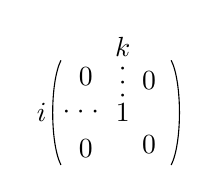
\begin{tikzpicture}[baseline=-0.5ex,x=0.7cm,y=0.7cm]
\draw (-1,0.95) .. controls (-1.2,0.55) and (-1.2,-0.55) .. (-1,-0.95);
\draw (1,0.95) .. controls (1.2,0.55) and (1.2,-0.55) .. (1,-0.95);
\node at (-0.55,0.65) {$0$};
\node at (0.6,0.58) {$0$};
\node at (-0.55,-0.65) {$0$};
\node at (0.6,-0.58) {$0$};
\node at (0.12,0) {$1$};
\node at (-0.9,0) {$\cdot$};
\node at (-0.64,0) {$\cdot$};
\node at (-0.38,0) {$\cdot$};
\node at (0.12,0.29) {$\cdot$};
\node at (0.12,0.54) {$\cdot$};
\node at (0.12,0.79) {$\cdot$};
\node at (-1.35,0) {$i$};
\node at (0.12,1.2) {$k$};
\end{tikzpicture}
\end{adjustbox}
— базис в пр-ве матриц
(1 на месте $i,k$)

% Tensor line: (450,2390,1170,2530), 4x. The n below the middle factor is visible.
\begin{equation*}
\sigma_n^{ik}=1\otimes\ldots\otimes\underset{n}{\sigma^{ik}}\otimes\ldots\otimes1
\end{equation*}

% Bottom: (55,2540,1900,3350), 2x;
% (215,2535,1150,2640), (235,2625,1650,2800), (575,2790,820,2950),
% (475,2970,1180,3100), (490,3190,1380,3300), 4x.
% Added close crops: (735,2630,985,2720), (440,2540,620,2630),
% (238,2630,530,2720), 6x.
Имеем \Unclear{GELFAND-P000818}{hamiltonian-abbrev}{кв. / лок.} гамильтониан.

Замолодчиков получил \underline{частные} решения (при разных $M$)

Используем их при $\underline{M=3}$, Получим
\begin{equation}
H=\sum_n\text{\Unclear{GELFAND-P000818}{eq14-crossing}{зачёркнуто, неразборчиво}}
(\vec{S}_n\,\vec{S}_{n+1})^2-2\vec{S}_n\,\vec{S}_{n+1}
\tag{14}
\end{equation}

$\underline{M=2}$ — изотр. ферромагн. Гейзенберга
\begin{equation}
H=\sum_n\vec{\sigma}_n\,\vec{\sigma}_{n+1}
\tag{15}
\end{equation}

спин $1/2$ — ничего больше инв. нет.

\SourcePage{GELFAND-P000819}{68}
% Original source: 2440 x 3480 pixels, directly inspected at native resolution.
% Wavy underlining in the source is represented by ordinary underlining below.
% Resolved close readings used source-pixel rectangles [x0,y0,x1,y1):
% label [2030,25,2410,150), 2x; representation note [340,245,1520,460), 2x;
% warning end [1450,570,2410,720), 2x; formula (17) [210,875,1390,1110), 2x,
% and dot on S [680,900,980,1060), 4x;
% second-neighbourhood wording [1400,1375,2430,1525), 2x;
% formula (18) factors [640,2010,1050,2240) and [820,2010,1230,2240), 2x;
% formula (2)' [545,2730,1490,2930), 2x, with [1010,2730,1230,2940), 3x;
% formula (20) [405,3050,1510,3320), 2x, with [1020,3050,1240,3280), 3x;
% comparison beta/gamma glyphs in (16) [380,154,965,270), 3x.
% Final punctuation checks: [970,2010,1460,2250), 3x, shows two low dots in (18);
% [310,1785,600,1895), 3x, shows no full stop after «Сущ»;
% [830,2630,1180,2740), 3x, shows two short horizontal strokes after (2).
% The two dots and two short strokes are retained as two visible marks.

В (14): $S^\alpha$ такие, что
\begin{equation*}
 [S^\alpha,S^\beta]=\varepsilon_{\alpha\beta\gamma}S^\gamma,
 \tag{16}
\end{equation*}
$S^\alpha$ --- \Unclear{GELFAND-P000819}{upper-rotation-abbreviation}{беск.} мал. поворот.

(предст. гр. $SO(3)$)

присоед. $=$ стандартное

Здесь нет параметров

$\underline{\underline{M=3}}\Rightarrow$ общего реш. нет.

(!) \underline{Неизвестно, как к гам. (14) добавить параметры,}
\underline{чтобы уложиться в сх. Замолодчикова.}

Эта схема сод. все вполне инт. квант. системы (2-мерные)

($\Rightarrow$ классические тоже после квазикласс. пред. перехода).

\begin{equation*}
 H=\sum_{n=1}^{N}\dot{S}_{ik}^{\alpha\beta}(0)
 \sigma_n^{i\beta}\sigma_{n+1}^{\alpha k};
 \tag{17}
\end{equation*}

\underline{Вопрос И.М.Г.}: соотн. на $S$ --- типа Маурера--Картана

(17) --- наиболее общ. вид гам. с взаимод. ближ. соседей.

Он \underline{всегда} облад. нетрив. интегралом, т.к. дифф. ур-я прод. до 2-й окрестности
\begin{equation*}
 S=S(0)+S'(0)\theta+\frac{S''(0)\theta^2}{2}
\end{equation*}
$S''$ восстанавливается.

$A_i(\theta)$ матрицы $\Rightarrow$ есть \underline{ассоциат.} автоматически

Сущ способ размножать алгебры.

Пусть нашли $S_{ik}^{\alpha\beta}$. Построим

(напр. $\underline{M=2}$)

\begin{equation*}
 \text{\Unclear{GELFAND-P000819}{eq18-l-indices}{$L^{ik}_{\vec{\alpha}\vec{\beta}}$; правка}}
 =S_{ij_1}^{\alpha_1\beta_1}
 S_{j_2j_3}^{\alpha_2\beta_2}.\, .
 S_{j_Nk}^{\alpha_N\beta_N}
 \qquad\text{(след не взяли)}
 \tag{18}
\end{equation*}

Получ. матрица
\begin{equation*}
 L=\begin{pmatrix}L_{11}&L_{12}\\L_{21}&L_{22}\end{pmatrix}
 =(L^{\alpha\beta})
 \tag{19}
\end{equation*}
элем. к-рой --- \underline{тоже матрицы}.

\Unclear{GELFAND-P000819}{lower-left-deletion}{Зачёркнутый знак перед «Соотнош.»: неразборчиво.}
Соотнош. типа (2) - - справедливы для матрицы $L$

\begin{equation*}
 S_{ik}^{\alpha\mu}S_{kj}^{\beta\nu}S_{\mu\gamma}^{\nu\delta}
 =S_{\beta\nu}^{\alpha\mu}S_{ik}^{\mu\gamma}S_{kj}^{\nu\delta}
 \tag*{(2)'}
\end{equation*}

$L^{ik}$ --- матр. $M^N\times M^N$ при всех $i,k$.

Есть соотношения:
\begin{equation*}
 \begin{array}{rccccccc}
 &L^{\alpha\mu}&L^{\beta\nu}&S_{\mu\gamma}^{\nu\delta}
 &=&S_{\beta\nu}^{\alpha\mu}&L^{\mu\gamma}&L^{\nu\delta}.\\
 \text{аргументы:}&\theta&\theta'&\theta-\theta'
 &&\theta-\theta'&\theta'&\theta
 \end{array}
 \tag{20}
\end{equation*}

\SourcePage{GELFAND-P000820}{unlabelled}
% Осмотрен оригинал 2440 x 3480; уверенно читаемого номера листа нет.
% Координаты (x0,y0,x1,y1): начало в левом верхнем углу,
% правая и нижняя границы исключены. head (325,30,1740,350), 3x.
Пусть теперь

\begin{equation*}
(21)\qquad A_{\alpha\mu}=L^{\alpha\mu}
\end{equation*}

Получится новая алгебра более выс. порядка

% grid (340,350,2070,690), 3x: пять вертикальных и пять горизонтальных линий.
\begin{center}
\begin{adjustbox}{max width=\linewidth}
\begin{tikzpicture}[x=1cm,y=1cm]
\draw (-0.12,0) -- (2.12,0);
\draw (-0.1,0.5) -- (2.06,0.5);
\draw (-0.12,1) -- (2.1,1);
\draw (-0.08,1.5) -- (2.15,1.54);
\draw (-0.12,2) -- (2.2,2.04);
\draw (0,-0.08) -- (0.06,2.1);
\draw (0.5,-0.08) -- (0.54,2.1);
\draw (1,-0.08) -- (1.03,2.08);
\draw (1.5,-0.06) -- (1.49,2.12);
\draw (2,-0.06) -- (2,2.12);
\node at (-0.8,1.02) {$n$};
\node at (1,-0.3) {$m$};
\node[anchor=west] at (2.9,1.15) {2-мерн. решетка, свернутая в тор.};
\end{tikzpicture}
\end{adjustbox}
\end{center}

% onsager (290,680,1860,950), 3x; pred-full (755,760,918,855), 8x.
Онзагер в 44г. --- 2-мерн. модель Изинга

---||--- 65г. --- \Unclear{GELFAND-P000820}{onsager-verb}{прид. / пред.}
коммут. трансфер-матрицу.

\begin{equation*}
\sigma_{n,m}=\pm1
\end{equation*}

Надо вычисл. сумму:

% sum (160,950,1980,1320), 3x.
\begin{equation*}
(22)\qquad
Z=\sum_{\{\sigma_{n,m}\}}
e^{J_1\sum\sigma_{n,m}\sigma_{n,m+1}+J_2\sum\sigma_{n,m}\sigma_{n+1,m}}
\end{equation*}
[В конце показателя степени зачёркнуто:
\Unclear{GELFAND-P000820}{exponent-cancellation}{неразборчиво}.]

% Abbreviation ближ.: (850,1320,1040,1410), 8x; no separate н established.
(взаимод. ближ. соседей)

Идея:

% idea (350,1320,2070,1805), 3x.
\begin{equation*}
(23)\qquad Z=\operatorname{Tr}T^N
\end{equation*}

% diagonal-dots (340,1580,655,1820), 6x.
\SourceFigure{GELFAND-P000820}{diagonal-dots}{Две параллельные наклонные линии, направленные снизу слева вверх вправо. На левой видны три кружка, на правой четыре; между линиями три отдельных кружка. Линия справа имеет небольшой разрыв перед верхним кружком. У верхнего кружка левой линии штрихи сливаются: требуется проверка формы этой отметки и наличия отдельного наконечника. Подписей возле кружков не видно.}

[Справа:] \underline{Онзагер:}
% Close reading: (1125,1590,1290,1695), 8x; terminal м agrees with nearby м.
идём по диагоналям

(по спинам промежут. диаг. суммируем)

% tail (155,1850,1340,2610), 3x; trace-note (400,1850,970,2030), 5x.
\begin{equation*}
(24)\qquad T_{\vec\alpha\,\vec\beta}=S_1\ldots S_n,
\end{equation*}

где

\begin{equation*}
(25)\qquad S_{ik}^{\alpha\beta}=
\begin{adjustbox}{max width=\linewidth}
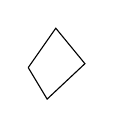
\begin{tikzpicture}[x=1cm,y=1cm,baseline=0cm]
\draw (0,0) -- (0.35,0.5) -- (0.72,0.05) -- (0.24,-0.4) -- (0,0);
\end{tikzpicture}
\end{adjustbox}
\end{equation*}

Получ. тр.-матр.\qquad $T(J_1,J_2)$

\underline{Утв.}

$T(J_1,J_2)$ коммут.
\Unclear{GELFAND-P000820}{bottom-fragment}{пр / при [запись обрывается]}

\end{document}
